%%%%%%%%%%%%%%%%%%%%%%% file template.tex %%%%%%%%%%%%%%%%%%%%%%%%%
%
% This is a template file for Proccedings 
%
% Copy it to a new file with a new name and use it as the basis
% for your article
%
%%%%%%%%%%%%%%%%%%%%%%%%   EDP Sciences  %%%%%%%%%%%%%%%%%%%%%%%%%%
%
\documentclass[proc]{edpsmath}
%
%\usepackage{amsfonts,graphicx,amssymb}%amsfonts pour les \mathbb
%\usepackage{amsmath,amsthm,amssymb}
%%%%%%%%%%%%%--PREAMBLE--%%%%%%%%%%%%%%%%%%
%%-----------------------------
%%         ...........
%%         your macros
\usepackage[frenchb,english]{babel}
\usepackage{macros}
\usepackage{tikz}
\usepackage{xcolor}
\usepackage[utf8]{inputenc}
\usepackage{amsmath,amsfonts,amssymb,amsthm,epsfig,epstopdf,array}
\usepackage{tikz}
\usetikzlibrary{matrix,arrows,decorations.pathmorphing}
\usepackage{caption}
\usepackage{pgfplots}
\usepackage{ulem}
\usepackage{pifont}% http://ctan.org/pkg/pifont
\usepackage{hyperref}
\usepackage{diagbox}
\usepackage{color}
\usepackage{placeins}
%\newenvironment{remark}[1][Remark]{\begin{trivlist}
%\item[\hskip \labelsep {\bfseries #1}]}{\end{trivlist}}
\newtheorem{theorem}{Theorem}[section]
\newtheorem{df}{Definition}[section]
\newtheorem{lemma}[theorem]{Lemma}
\newtheorem{remark}[theorem]{Remark}
\definecolor{blue}{rgb}{0.30,0.8,1}
\definecolor{red}{rgb}{1,0.3,0.3}
%\usetikzlibrary{positioning,shapes,shadows,arrows}

%%         ...........
%%-------------------------%%----
%%%%%%%%%%%%%%%--BODY--%%%%%%%%%%%%%%%%%%

\begin{document}
\newcommand{\urev}[1]{{\color{red}#1}}
\newcommand{\mrev}[1]{{\color{blue}#1}}

%%-----------------------------
%%      the top matter
%%-----------------------------
\title{A numerical study of the
	solution of X-Mode equations around the hybrid resonance}
\thanks{\rm The authors acknowledge 
	the support
	of ANR under contract ANR-12-BS01-0006-01. Moreover,  
	this work was carried out within the framework of the European Fusion Development Agreement and 
	the French Research Federation for Fusion Studies. 
	It is supported by the European Communities under the contract of Association between Euratom and CEA. 
	The views and opinions expressed herein do not necessarily reflect those of the European Commission.} %\thanks{...}\thanks{...}% At most 5 thanks
%
\author{C\'eline Caldini-Queiros}\address{Max Planck Institute für PlasmaPhysik, Garching bei München, Germany}
\author{Bruno Despr\'es}\address{Sorbonne Universit\'es, UPMC Univ Paris 06, UMR 7598, Laboratoire Jacques-Louis Lions, F-75005, Paris, France}
\author{Lise-Marie Imbert-Gérard}\address{Courant Institute of Mathematical Sciences, New York University}
\author{Maryna Kachanovska}\address{POEMS, INRIA, ENSTA ParisTech, Palaiseau, France}


%
%\dedicated{\it Dedicated to Maurice Dupont} %if necessary
%
\begin{abstract}
Hybrid resonance is a physical phenomenon 
that appears for example in the heating of plasma, 
and as such is of interest in the developing of new sources of energy, 
e.g. in the ITER project. In this paper we focus on the non-regularity of
the solutions of Maxwell equations in plasmas 
under strong background magnetic field. 
Our purpose here is two-fold. 
On one hand we investigate the finite element approximation of the one-dimensional problem 
written in the frequency domain, 
and on the other hand we study the finite difference approximation 
of the one-dimensional time dependant problem. 
We compare the results of these two differents methods in the context of limiting absorption and limiting amplitude principles.
\end{abstract}
%
\begin{resume} 
La r\'esonnance hybride est un ph\'enom\`ene physique qui apparait par exemple lorsque l'on chauffe un plasma, et 
ainsi est d'int\'er\^et scientifique dans le cadre du d\'eveloppement  du projet ITER. Dans ce papier, nous nous concentrons sur des solutions faiblement r\'eguli\`eres des \'equations de Maxwell pour les plasmas sous l'influence de champ magn\'etiques forts. Notre but principal est ici double. D'un c\^ot\'e nous \'evaluons l'approximation 
num\'erique \`a l'aide d'\'el\'ements finis de la formulation 
fr\'equentielle, et de l'autre nous \'etudions les solutions r\'esonnantes dans le domaine temporelle, \`a l'aide de deux approximation diff\'erences finies diff\'erentes. Nous comparons ensuite les r\'esultats ainsi obtenus avec ceux donn\'es dans le domaine fr\'equentiel. Ceci est fait en regardant num\'eriquement les principes d'amplitude et d'absorption limite.



\end{resume}
%
%
\maketitle
%\textcolor{red}{should we add Olivier Lafitte and Remi Sart anywhere in the proceeding ?}\\

\section{Introduction}
Modelling various phenomena in plasmas is of practical importance for developing new sources of energy 
based on plasma fusion, see the ITER project\footnote{www.iter.org}. 
In particular, this article concentrates on studying a phenomenon of hybrid resonance \cite{Stix}, 
which is observed in experiments \cite{reflectometers_2006, reflectometers_2010, Dumont_2005} and 
mathematically is described as the non-regularity of
the solutions of Maxwell equations in plasmas under strong background magnetic field \cite{Despres_2014}. 
The energy deposit is resonant and may exceed by far the energy 
exchange which occurs in Landau damping \cite{Freidberg_2007,Mouhot_2011}. 
Contrary to the Landau damping, however, 
hybrid resonance appears in a simpler model coupling 
fluid equations with the non electrostatic part of Maxwell equations.


We consider the model of cold plasma of \cite{Stix} which is described by the non-stationary Maxwell system  
\begin{align}
-\varepsilon_0 \partial_t \E + \curl\, \Hbf = \J\\
\mu_0 \partial_t \Hbf + \curl\, \E = 0
\end{align}
coupled with a linear current in two dimensions $\J = eN_e \ubf_e$, and takes into account the friction  $\nu$ between particles
\be
m_e \partial_t \ubf_e =e (\E +\ubf_e \nabla B_0) -m_e \nu \ubf_e. \label{eq:electronmove}
\ee
The unknows are the electromagnetic field $(\E,\Hbf)$ with the usual notation $\Hbf = \B/\mu_0$, 
the electronic current $\J$, 
and the velocity of electrons $\ubf_e$. Here $B_0$ is the background magnetic field, typically assumed to be uniform in time and space.  
We denote by $e<0$ the value of the charge of electrons, $m_e$ the electron mass and $N_e$ the electron density that in general 
depends on spatial variables and is uniform in time. 
Without loss of generality, we set $\mathbf{B}_0=\left(0,\; 0,\; B_0\right)$, which allows to obtain the following system of equations 
\begin{align}
\label{eq:main_model}
\begin{split}
\epsilon_0\partial_t E_{x}-\partial_y H=-eN_e u_x,\\
\epsilon_0\partial_t E_{y}+\partial_x H=-eN_e u_y,\\
\mu_0\partial_t H+\partial_x E_y-\partial_y E_x=0,\\
m_e\partial_t u_x=eE_x+eu_yB_0-\nu m_e u_x,\\
m_e\partial_t u_y=eE_y-eu_xB_0-\nu m_e u_y
\end{split}
\end{align}
posed in $[-L,\; \mathbb{R}]\times \mathbb{R}$. 
The energy of this system for $\nu=0$ in a domain $\Omega$ can be expressed as \cite{stable_yee_plasma_current}
\begin{align*}
{\mathcal E}(t)= \int_\Omega \left(
\frac{\epsilon_0 |\E(t,\x)|^2}{2}+\frac{ |\B(t,\x)|^2}{2\mu_0}+\frac{m_e|\J (t,\x)|}{2|e|N_e(\x)} \mathrm{d}\x.
\right)
\end{align*}
From this it can be seen that if the electron density $N_e(x)$ vanishes, 
the energy blows up~\cite{stable_yee_plasma_current}. 
Mathematically, this effect was recently investigated in \cite{Despres_2014}, 
in particular, it was shown that the electric field $E_x$ in this case is no longer square 
integrable, and explicit estimates on the behaviour of the solutions of \eqref{eq:main_model} in 1D were given. 

In this work we look at a simplification of this model obtained after 
the Fourier transform of (\ref{eq:main_model}) in $y$. 



The goal of this article is two-fold. 
First, we investigate the finite element approximation of the 1D 
problem \eqref{eq:main_model} written in the frequency domain ($\partial_t\rightarrow -i\omega$).
\mrev{More precisely, 
\begin{align*}
%\label{eq:main_frequency_domain_1}
\operatorname{curl}\operatorname{curl}\hat{\mathbf{E}}-
\epsilon(\omega)\hat{\mathbf{E}}=0,\\
\epsilon(\omega)=\left(
\begin{matrix}
 \tilde{\alpha} & i\tilde{\delta} \\
 -i\tilde{\delta}  & \tilde{\alpha}
\end{matrix}
\right),\\
\tilde{\alpha}(\omega)=\frac{\omega^2}{c^2}\left(1-\frac{\tilde{\omega}\omega_p^2}{\omega(\tilde{\omega}^2-\omega_c^2)}\right),\qquad 
\tilde{\delta}(\omega)=\frac{\omega_c\omega_p^2}{\omega(\tilde{\omega}^2-\omega_c^2)},\\
\tilde{\omega}=\omega+i\nu,\qquad \omega_c=\mrev{\frac{eB_0}{m_e}},\qquad \omega_p^2=\frac{e^2 N_e}{\epsilon_0 m_e}.
\end{align*}
After expansion in $\nu\rightarrow 0$ and keeping lower-order terms only
\begin{align*}
 \tilde{\alpha}(\omega)=\alpha(\omega)+i\nu\frac{\omega_p^2(\omega^2+\omega_c^2)}{(\omega^2-\omega_c^2)^2}\frac{\omega^2}{c^2},\qquad \alpha(\omega)=\frac{\omega^2}{c^2}\left(1-\frac{\omega_p^2}{\omega^2-\omega_c^2}\right),\\
 \tilde{\delta}(\omega)=\delta(\omega)-\frac{2i\omega^3\nu}{c^2(\omega^2-\omega_c^2)^2},\qquad \delta(\omega)=\frac{\omega\omega_c\omega_p^2}{c^2(\omega^2-\omega_c^2)}.
\end{align*}
Then the limiting absorption principle can be obtained leaving only the diagonal terms in the above expansion (see \cite{Despres_2014}):
\begin{align}
\label{eq:main_frequency_domain}
\operatorname{curl}\operatorname{curl}\hat{\mathbf{E}}-\frac{\omega^2}{c^2}
\left(\epsilon_0(\omega)+\nu Id\right)\hat{\mathbf{E}}=0,\\
\nonumber
\epsilon_0(\omega)=\left(
\begin{matrix}
 \alpha & i\delta \\
 -i\delta & \alpha 
\end{matrix}
\right)
\end{align}
}
\urev{Additionally, we assume $\alpha(\omega)$ and $\delta(\omega)$ be sufficiently smooth, i.e. bounded and continuous in  
$\left[-L,\; \mathbb{R}\right)$.}
In particular, we again investigate this problem in one dimension, performing the Fourier transform in $y$.
We prove the well-posedness of this problem for $\nu>0$ in Section~\ref{sec:wellposedness} and 
demonstrate that the use of higher-order (P1) finite elements allows to approximate the singularity 
of the solution fairly well (Section \ref{sec:freq_dep}). 
Second, we consider the case $\nu\rightarrow 0$, and study the limiting amplitude solution 
$\lim\limits_{t\rightarrow +\infty}\lim\limits_{\nu\rightarrow 0}\mathbf{E}(t)$ obtained with the help of 
the FDTD discretization of \eqref{eq:main_model}, suggested in \cite{stable_yee_plasma_current}. 
We compare this result with 
$\hat{\mathbf{E}}\mathrm{e}^{i\omega t}$, computed in the frequency domain, for $\nu\rightarrow 0$, i.e.
$\lim\limits_{\nu\rightarrow 0}\lim\limits_{t\rightarrow+\infty}\mathbf{E}(t)$.

To our knowledge, such numerical studies have not been performed in the existing literature. 

To solve the problem (\ref{eq:main_model}) numerically, we equip it with the following boundary conditions.
At the left boundary of the domain we choose Robin boundary conditions 
\be
-curl \E -\imath \lambda\E \wedge \n = g_{inc} = -curl \E_{inc} -\imath\lambda\E_{inc} \wedge \n,
\ee
where $\E_{inc} = \exp \left(\imath \lambda x\right)\begin{pmatrix} E_1\\ E_2 \end{pmatrix}$. We truncate the domain 
$(-L,\; \mathbb{R})$ to $(-L,\; H)$ and set on the right boundary $\operatorname{curl} \E = 0$. 
\begin{remark}
	When modelling antennas in plasma physics, in such applications as ITER, 
	a good choice of boundary condition could be $\lambda = \sqrt{\alpha(-L)}$
\end{remark}

\section{Frequency domain study}
The goal of this section is to review the connection between the system (\ref{eq:main_system}), its frequency domain counterpart and 
the regularized problem (\ref{eq:seq_regularized}). 

In the frequency domain, the velocity can be eliminated to obtain a simpler system under the form
of  Maxwell equations with the cold plasma dielectric tensor \cite{Stix,Despres_2014}, more precisely
\urev{
\bealn
%\label{eq:main_frequency_domain_1}
\operatorname{curl}\operatorname{curl}\hat{\mathbf{E}}-
\frac{\omega^2}{c^2}\underline{\varepsilon}^{\nu}_{\omega}(\mathbf{r})\hat{\mathbf{E}}=0,\\
\underline{\varepsilon}^{\nu}_{\omega}(\mathbf{r})=\left(
\begin{matrix}
 \alpha^{\nu}_{\omega}(\mathbf{r}) & i\delta^{\nu}_{\omega}(\mathbf{r}) \\
 -i\delta^{\nu}_{\omega}(\mathbf{r}) & \alpha^{\nu}_{\omega}(\mathbf{r})
\end{matrix}
\right),\qquad 
 \alpha^{\nu}_{\omega}(\mathbf{r})=\frac{\omega^2}{c^2}\left(1-\frac{\omega_{\nu}\omega_p^2(\mathbf{r})}{\omega(\omega_{\nu}^2-\omega_c^2(\mathbf{r}))}\right),\qquad 
\delta^{\nu}_{\omega}(\mathbf{r})=\frac{\omega_c(\mathbf{r})\omega_p^2(\mathbf{r})}{\omega(\omega_{\nu}^2-\omega_c^2(\mathbf{r}))},
\eealn
}
\mrev{where the frequency 
$\omega_{\nu}=\omega+i\nu$ is shifted in the complex plane. Note that neither cyclotron, nor hybrid resonances occur in the problem with the dielectric tensor $\epsilon^{\nu}_{\omega}(\mathbf{r}), \; \nu>0,$ (since all parameters are real). Hence 
the choice of the non-zero plasma friction $\nu>0$ can be viewed as a regularization of the problem. }

\mrev{
The series expansion as $\nu\rightarrow 0$ gives at leading orders
\bealn
 \alpha^{\nu}_{\omega}=\alpha_{\omega}+i\nu\frac{\omega_p^2(\omega^2+\omega_c^2)}{(\omega^2-\omega_c^2)^2}=\alpha_{\omega}+i\nu D_{\alpha},\\
 \delta^{\nu}_{\omega}=\delta_{\omega}-i\nu\frac{2\omega}{(\omega^2-\omega_c^2)^2}=\alpha_{\omega}+i\nu D_{\delta},
\eealn
where $\alpha_{\omega},\;\delta_{\omega}$ are defined by (\ref{eq:alpha_delta}). In the frequency domain one thus can consider 
the following regularization of the cold plasma dielectric tensor of (\ref{eq:main_frequency_domain}):
\begin{align*}
\underline{\varepsilon}^{\nu}_{\omega}\approx \underline{\varepsilon}^0_{\omega}+i\nu \left(
 \begin{matrix}
  D_{\alpha} & D_{\delta}\\
  -D_{\delta} & D_{\alpha}
 \end{matrix}
\right).
\end{align*}
However, as demonstrated in \cite{singular_solutions} for the 1D setting, a significantly simpler regularization (considered in \cite{Despres_2014})
\ben
\epsilon^{\nu}_{\omega}(\mathbf{r})\approx \epsilon^{0}_{\omega}(\mathbf{r})+i\nu \mathbb{E}
\een
yields the same solution as $\nu\rightarrow 0$. }
%We finally obtain a simpler equation \cite{Despres_2014} 


Thus, applying the above process to (\ref{eq:main_model}), we obtain, see also \cite{Despres_2014},
\begin{align}
\label{eq:main_frequency_domain}
\left(
\begin{matrix}
 i\theta \partial_x \hat{E}_y+\theta^2 \hat{E}_x\\
 i\theta \partial_x \hat{E}_x -\partial_x^2 \hat{E}_y
\end{matrix}
\right)-\frac{\omega^2}{c^2}
\left(\epsilon^{0}_{\omega}(x)+\nu \mathbb{E}\right)\left(
\begin{matrix}
 \hat{E}_x\\
 \hat{E}_y
\end{matrix}
\right)
=0,\\
\label{eq:epsilon_0}
\epsilon^0_{\omega}(x)=\left(
\begin{matrix}
 \alpha_{\omega}(x) & i\delta^{0}(x) \\
 -i\delta_{\omega}(x) & \alpha^{0}(x)
\end{matrix}
\right)=
\left(
\begin{matrix}
 \alpha(x) & i\delta(x) \\
 -i\delta(x) & \alpha(x)
\end{matrix}
\right).
\end{align}
\urev{
From now on we will assume the following assumption to hold.
\begin{assumption}
\label{assumption:smooth}
The coefficients  $\alpha(x)$ and $\delta(x)$ are assumed to be sufficiently smooth, i.e. bounded and continuous in  
$\left[-L,\; H\right]$.
\end{assumption}
It can be ensured e.g. by requiring the continuity of $N_e(x), B_0(x) \in [-L,\;H]$ and the absence of the cyclotron resonance, i.e. for all $x$ $|\omega_c^2(x)-\omega^2(x)|>c>0$ on this interval. 
}

\begin{remark}
For the time domain problem (\ref{eq:main_model}) the choice of the sign of $\nu>0$ is of crucial importance for the stability of the problem. 
In the frequency domain, as we can see from above and from \cite{Despres_2014,LMIG_thesis}, the sign 
of the parameter $\nu$ can be chosen arbitrarily to regularize the problem. However, as demonstrated in the above references, as $\nu\rightarrow 0\pm$, the 
limiting solutions differ, though both exhibit the singularity in the point of the hybrid resonance.  
\end{remark}
%}

%%%%%%%%%%%%%%%%%%%%%% 
\subsection{1D case}
%%%%%%%%%%%%%%%%%%%%%% 
\label{sec:wellposedness}

In order to reduce problem \eqref{eq:main_frequency_domain} to one dimension, perform a Fourier transform in the $y$ variable, 
denoting by $\theta$ the corresponding Fourier variable. 
After introducing $\Omega=(-L,\; H)\subset \mathbb R$ and defining the function space of the problem  $\mathbf{V}=L^{2}(\Omega)\times H^{1}(\Omega)$, 
equipped with the norm
\ben
 \|\mathbf{v}\|_{\mathbf{V}}^2= \|v_1\|_{L^{2}(\Omega)}^2+\|v_2\|_{H^{1}(\Omega)}^2,
\een
the resulting one-dimensional system can be rewritten in the following variational form:
\begin{align}
\label{vf1dcase}
\begin{array}{l}
\displaystyle \int_{-L}^H (E_y' -\imath\theta E_x)\overline{(\tilde E_y' -\imath \theta \tilde E_x)} - \int_{-L}^H (\eps_0 +\imath\nu Id) \E \cdot \overline{\tilde \E}
%\\ \displaystyle 
 - \imath \lambda E_y (-L)\overline{ \tilde E_y (-L)} = -g_{inc} (-L) \overline{( \tilde E_y(-L) )},
\end{array}\\
\nonumber
\text{ for all } \tilde{\mathbf{E}}=(\tilde E_x,\tilde E_y)\in \mathbf{V}.
\end{align}
Recall that here $\lambda\geq 0$. 
%=\omega\geq 0$. 
Let us remark that in this and further sections, where it is not ambiguous, we will use the notation $E_{x,y}$ instead of $\hat{E}_{x,y}$ for convenience.

The above can be reformulated as 
\be
a\left(\mathbf{u},\mathbf{v}\right)=l(\mathbf{v}), \; \text{ for all }\mathbf{v}\in \mathbf{V},
\ee
with a bilinear form $a$ and a linear form $l$:
\be
a(\ubf,\vbf) = a_1 (\ubf,\vbf) +\imath a_2(\ubf,\vbf)\  \text{ and } \  l(\vbf) = -g_{inc} (-L) \overline{(v_2(-L) )} 
\ee
where $a_1= a_1^*$ and $a_2=a_2^*$ are hermitian
\be
\left\{\begin{array}{l}
	a_1(\ubf,\vbf) = \int_{-L}^H (u_2' -\imath\theta u_1)\overline{(v_2' -\imath \theta v_1)} - \int_{-L}^H \eps_0 \ubf\cdot \overline{\vbf}, 
	\\ a_2(\ubf,\vbf) = -\nu \int_{-L}^H  \ubf\cdot \overline{\vbf} - \lambda u_2 (-L) \overline{v_2 (-L)} , 
\end{array}\right.
\ee
The unknown is $\ubf=(E_x,E_y)=(u_1,u_2)$ and $\vbf$ is a test function.

\urev{
Let us denote the spectral radius of $\eps_0$ by $\heps =  \|\rho(\eps_0)\|_{L^{\infty}[-L,\;H]}$. 
By Assumption \ref{assumption:smooth}, the spectral radius $\heps=\max\left(\|\alpha+\delta^2\|_{L^{\infty}[-L,\;H]}, \|\alpha-\delta^2\|_{L^{\infty}[-L,\;H]}\right)$ 
is bounded.}
%\end{df}

We now prove the following result.

\begin{lemma}
\label{lemma:well_posedness}
Provided that Assumption \ref{assumption:smooth} holds, the bilinear form 
\ben
 a(\ubf,\vbf):  \mathbf{V}\times \mathbf{V}\rightarrow \mathbb{C}
\een
is continuous and coercive for all $\nu\neq 0$: for all $\ubf,\vbf\in \mathbf{V}$ it holds that
\bealn
\label{eq:bilinear_cont}
\left\{\begin{array}{l}
\Re\left(\mathrm{e}^{i\alpha_{\nu}}a(\ubf,\ubf)\right)\geq \frac{|\nu|}{\sqrt{(\heps+\theta^2+1)^2+\nu^2}}\left(\frac{1}{2}\|u_2'\|^2_{L^2}  + \| \ubf \|_{L^2}^2\right),\; 
\text{ for some $\alpha_{\nu}\in\left(-\frac{\pi}{2}, 0\right)\cup \left(0,\frac{\pi}{2}\right)$},\\
|a(\ubf,\vbf)|\leq C \|\ubf\|_{\mathbf{V}}\|\vbf\|_{\mathbf{V}},
\end{array}\right.
\eealn
where $C>0$ does not depend on $\nu$. The problem~\eqref{vf1dcase} is well-posed in $\mathbf{V}$.

\end{lemma}
%\textcolor{red}{!!!! redo coercivity computations !!!}
\begin{proof}
	The boundedness of $a$ is obvious using the continuous embedding in dimension
	one  $H_1(\Omega)\subset C^0(\overline \Omega)$. Let us focus on the proof of coercivity. 
	Without loss of generality let us assume that $\nu>0$. We denote $\heps =  \|\rho(\eps_0)\|_{L^\infty}$, the spectral radius of $\eps_0$ so that
	$\heps Id- \eps_0 $ is a non negative hermitian matrix.
	Therefore
	\be 
	a_1(\ubf,\ubf) + \heps\|\ubf\|^2_{L^2}= \|u_2' - \imath \theta u_1 \|^2_{L^2} + \left( (\heps Id - \eps_0 ) \ubf, \overline{\ubf} \right)  \geq \|u_2 ' - \imath \theta u_1 \|_{L^ 2}^ 2
	\geq \frac12 \|u_2 '  \|_{L^ 2}^ 2 -
	\theta ^2 \| u_1 \|_{L^ 2}^ 2.
	\ee
	Thus one can write
	$
	a_1(\ubf,\ubf)  \geq \frac{1}{2}\|u_2'\|^2_{L^2}-  (\heps  +  \theta^2) \| \ubf \|_{L^2}^2$.
	One also has that
	$
	a_2 (\ubf ,\ubf) \leq -\nu \| \ubf \|_{L^2}^2$. 
	Therefore
	\ben
	a_1(\ubf,\ubf)-\frac{\heps  +  \theta^2 + 1 }\nu a_2(\ubf,\ubf)\geq \frac{1}{2}\|u_2'\|^2_{L^2}  + \| \ubf \|_{L^2}^2,
	\een
	or, introducing $\alpha_{\nu}=\arccos\frac{1}{\sqrt{1+\left(\heps+\theta^2+1\right)^2\nu^{-2}}}$, this is equivalent to 
	\ben
	\Re\left(\mathrm{e}^{i\alpha_{\nu}}a(\ubf,\ubf)\right)\geq 
	\frac{1}{\sqrt{1+\left(\heps+\theta^2+1\right)^2\nu^{-2}}} \left(\frac{1}{2}\|u_2'\|^2_{L^2}  + \| \ubf \|_{L^2}^2\right)\\
	\geq \frac{\nu}{\sqrt{(\heps+\theta^2+1)^2+\nu^2}}\left(\frac{1}{2}\|u_2'\|^2_{L^2}  + \| \ubf \|_{L^2}^2\right).
	\een
	The problem \eqref{vf1dcase} is uniquely solvable thanks to Lax-Milgram theorem.
\end{proof}


\begin{remark} 
\label{remark:other}
The above proof is not optimal in the case when $\left|\alpha(x)\right|>c>0$ for $c>0$ on the whole interval $[-L,\; H]$, at least 
for the case $\theta=0$. In this case the problem (\ref{eq:var_form2}) is well-posed for $\nu=0$. More precisely, it can be written 
as a system of two equations, where the first equation (for $E_y$) is the variational formulation for the Helmholtz equation 
with the variable coefficient $k^2=(\alpha(x)-\frac{\delta^2}{\alpha(x)})$, and the second equation 
\begin{align*}
  \left(E_x,u\right)=-\left(\frac{i\delta}{\alpha(x)}E_y,u\right),\; \text{ for all } u\in L^{2}(\Omega), 
\end{align*}
uniquely defines $E_x\in L^{2}(\Omega)$. The well-posedness of the former problem, with additional assumptions on boundary conditions and smoothness of the coefficients, 
was demonstrated in \cite{LMIG_thesis}. Provided the solution $E_y\in H^{1}(\Omega)$, we can obtain $E_x$ from the second equation.

%%Let us consider the problem (\ref{eq:var_form2}) for $\nu=0,\; \theta=0$, which, after testing it 
%%with $(\tilde{E}_x,\; 0)$ and $(0,\; \tilde{E}_y)$ from $\mathbf{V}$, can be rewritten as, see also (\ref{eq:epsilon_0})
%%\begin{align}
%%\label{eq:full_var}
%%\begin{split}
%%\int_{-L}^H \left(\alpha E_x+i\delta E_y \right)_{1} \overline{\tilde E}_{x}&=0,\; \text{ for all }\tilde{E}_x\in L^{2}(\Omega), \;\\
%%\displaystyle \int_{-L}^H E_y'\tilde {E_y'} - \int_{-L}^H\left( -i\delta E_x+\alpha E_y \right)_{2}\overline{\tilde{E}}_{y}
%%  - \imath \lambda E_y (-L) \overline{\tilde E_y} (-L) &= -g_{inc} (-L) \overline{( \tilde E_y(-L) )},\\
%%  \text{ for all }  \tilde{E}_{y}\in H^{1}(\Omega).
%%  \end{split}
%%\end{align}
%%The first equation of the above can be rewritten as 
%%\ben
%% \left(E_x,\alpha \tilde{E}_x\right)=-\left(i\delta E_y,  \tilde{E}_x\right).
%%\een
%%If the multiplication operator $M_{\alpha}$ defined as $M_{\alpha}\psi=\frac{1}{\alpha}\psi$ is an isomorphism from $L^{2}([-L,\;H])$ to $L^{2}([-L,\;H])$ (this is true if e.g.
%%$\alpha \in C_{0}([-L,\;H])$ and $|\alpha(x)|>c>0$, for some $c>0$, on the whole interval), this equation is equivalent to 
%%\begin{align}
%%\label{eq:mult_eq}
%%  \left(E_x,u\right)=-\left(\frac{i\delta}{\alpha}E_y,u\right),\; \text{ for all } u\in L^{2}(\Omega). 
%%\end{align}

%%Choosing in the above $u=-i\delta \tilde{E}_y \in L^{2}(\Omega)$ and adding it to the second equation of (\ref{eq:full_var}), we obtain
%%\bealn
%% \displaystyle \int_{-L}^H E_y'\tilde {E_y'} - \int_{-L}^H (\alpha-\frac{\delta^2}{\alpha})E_y \overline{\tilde{E}}_{y}
%%  - \imath \lambda E_y (-L) \overline{\tilde E_y} (-L) &= -g_{inc} (-L) \overline{( \tilde E_y(-L) )},\\
%%  \text{ for all } \tilde{E}_{y}\in H^{1}(\Omega). \nonumber
%%\eealn
%%Thus we obtain the variational formulation for $E_y$, or the variational formulation for the Helmholtz equation. The well-posedness 
%%of this problem, with additional assumptions on boundary conditions and smoothness of the coefficients, 
%%had been demonstrated in \cite{LMIG_thesis}. Provided the solution $E_y\in H^{1}(\Omega)$, we can obtain $E_x$ from the equation (\ref{eq:mult_eq}).
\end{remark}

%\subsection{2D case}
%%%%%%%%%%%%%%%%%%%%%% 


%%%%%%%%%%%%%%%%%%%%%% 
%\textcolor{red}{!!!!!!!!!!!!!!!! TODO : deal with this part !!!!!!!!!!!}
%$curl$ ibp formula
%\be
%\int_\Omega \curl u \cdot \f = \int_\Omega u\ curl \f + \int_\Gamma u (\f \wedge \n)
%\ee
%\be
%\int_\Omega curl \E \cdot \overline{curl \tilde \E} - \int_\Omega \eps \E \cdot \overline{\tilde \E} + \int _\Gamma curl \E \overline{\left( \tilde \E\wedge \n \right)} d\sigma = 0
%\ee
%\be
%\begin{array}{l}
%\displaystyle \int_\Omega curl \E \cdot \overline{curl \tilde \E} - \int_\Omega (\eps_0+i\nu Id) \E \cdot \overline{\tilde \E} - \int _{\{x=-L\}} \imath \sqrt{\alpha(-L)}(\E\wedge \n) \overline{\left( \tilde \E\wedge \n \right)} d\sigma 
%\\ \displaystyle \phantom{ fffffffff}= \int_{\{x=-L\}} g_{inc}  \overline{\left( \tilde \E\wedge \n \right)} d\sigma
%\end{array}\ee
%\textcolor{red}{!!!!!!!!!!!!!!!!!!!!!!!!!!!!!!!!!!!}


%%%%%%%%%%%%%%%%%%%%
\subsection{Discretization of the Frequency Domain Problem}
\label{sec:discr}
Testing the variational formulation (\ref{vf1dcase}) with $(\tilde E_x,0)$ and $(0,\; \tilde{E}_y)\in\mathbf{V}(\Omega)$ and using 
an explicit expression for the tensor of the dielectric permittivity (\ref{eq:epsilon_0}), we can rewrite it as a system of two equations
%\begin{align*}
%\begin{split}
%i\theta \displaystyle \int_{-L}^H (E_y' -\imath\theta E_x)\overline{\tilde E_x} - \int_{-L}^H \left((\epsilon_0 +\imath\nu \operatorname{Id}) \E\right)_{1} \overline{\tilde E}_{x}
%&=0,\\
%\displaystyle \int_{-L}^H (E_y' -\imath\theta E_x)\tilde {E_y'} - \int_{-L}^H\left( (\epsilon_0 +\imath\nu\operatorname{Id}) \E\right)_{2}\overline{\tilde{E}}_{y}
%  - \imath \lambda E_y (-L) \tilde E_y (-L) &= -g_{inc} (-L) \overline{( \tilde E_y(-L) )},\\
%  \text{ for all } \tilde E_x\in L^{2}(\Omega), \; \tilde{E}_{y}\in H^{1}(\Omega).
%  \end{split}
%\end{align*}
%Using the explicit expression for the dielectric permittivity tensor in the above, it yields: 

\begin{align}
\label{eq:var_form2}
\begin{split}
 i\theta \displaystyle \int_{-L}^H (E_y' -\imath\theta E_x)\overline{\tilde E_x} - 
 \int_{-L}^H \left((\alpha+i\nu)E_x+\imath\delta E_y\right)_{1} \overline{\tilde E}_{x}
&=0,\\
\int_{-L}^H (E_y' -\imath\theta E_x)\tilde {E_y'} -
\int_{-L}^H\left( -\imath \delta E_x+(\alpha+i\nu) E_y\right)_{2}\overline{\tilde{E}}_{y}
  - \imath \lambda E_y (-L) \tilde E_y (-L) &= -g_{inc} (-L) \overline{( \tilde E_y(-L) )},\\
 \text{ for all } \tilde E_x\in L^{2}(\Omega), \; \tilde{E}_{y}\in H^{1}(\Omega).
  \end{split}
\end{align}
Let us introduce two basis function spaces $V_{E_x}=\{\psi_{j}\}_{j=1}^{N_{1}}$ and $V_{E_{y}}=\{\phi_{i}\}_{i=1}^{N_{2}}$. 
%We look for the solution of the problem (\ref{eq:var_form2}) in the form:
We discretize problem (\ref{eq:var_form2}) as:
\ben
E_x=\sum\limits_{k=1}^{N_{1}}e_{xk}\psi_{k},\qquad E_{y}=\sum\limits_{k=1}^{N_{2}}e_{yk}\phi_{k}.
\een

% Substituting $\tilde{E}_{x}=\psi_{m}, \; m=1,\ldots,N_{1}$ and $\tilde{E}_{y}=0$ into the variational formulation (\ref{}), we obtain:
% \begin{align*}
% i\theta\sum\limits_{k=1}^{N_{2}}e_{2k}\int\limits_{-L}^{H}\phi'_{k}\bar{\psi}_{m}dx+\theta^2\sum\limits_{k=1}^{N_{1}}e_{1k}\int\limits_{-L}^{H}\psi_{k}\bar{\psi}_{m}dx\\
% -\sum\limits_{k=1}^{N_{1}}e_{1k}\int\limits_{-L}^{H}(\alpha(x)+i\nu)\psi_{k}\bar{\psi}_{m}dx-i\sum\limits_{1}^{N_{2}}e_{2k}\int\limits_{-L}^{H}\delta(x)\phi_{k}(x)\bar{\psi}_{m}dx=0.
% \end{align*}
% Similarly, for $\tilde{E}_{x}=0$ and $\tilde{E}_{y}=\phi_{\ell},\; \ell=1,\ldots, N_{2}$:
% \begin{align*}
% \sum\limits_{k=1}^{N_{2}}e_{2k}\int\limits_{-L}^{H}\phi'_{k}(x)\bar{\phi}'_{\ell}(x)dx-i\theta\sum\limits_{k=1}^{N_{1}}e_{1k}\int\limits_{-L}^{H}\psi_{k}(x)\bar{\phi}'_{\ell}(x)dx\\
% +i
% \sum\limits_{k=1}^{N_{1}}e_{1k}\int\limits_{-L}^{H}\delta(x)\psi_{k}\bar{\phi}_{m}dx-\sum\limits_{k=1}^{N_{2}}e_{2k}\int\limits_{-L}^{H}(\alpha(x)+i\nu)\phi_{k}\bar{\phi}_{m}dx\\
% -
% i\lambda\sum\limits_{k=1}^{N_{2}}e_{2k}\phi_{k}(-L)\bar{\phi}_{m}(-L)=-g_{inc}(x)\bar{\phi}_{m}(-L).
% \end{align*}
Introducing the notation
\bealn
\left(K^{\psi,\phi'}\right)_{mk}=\int\limits_{-L}^{H}\bar{\psi}_{m}\phi'_{k}dx,\qquad \left(M^{\psi}\right)_{mk}=\int\limits_{-L}^{H}\psi_{k}\bar{\psi}_{m}dx, \qquad 
\left(M^{\alpha,\psi}\right)_{mk}=\int\limits_{-L}^{H}(\alpha(x)+i\nu)\psi_{m}\bar{\psi}_{k}dx,\\
\left(M^{\delta,\psi,\phi}\right)_{mk}=\int\limits_{-L}^{H}\delta(x)\bar{\psi}_{m}\phi_{k}dx, \qquad 
K_{\ell k}=\int\limits_{-L}^{H}\phi'_{k}(x)\bar{\phi}'_{\ell}(x)dx,\qquad
\left(M^{\alpha,\phi}\right)_{\ell k}=\int\limits_{-L}^{H}(\alpha(x)+i\nu)\bar{\phi}_{\ell}\phi_{k}dx,\\
I_{km}^{\Gamma}=\bar{\phi}_{m}(-L)\phi_{k}(-L), \\
\boldsymbol{e}_{x}=\left(e_{11},\ldots,e_{1 N_{1}}\right)^{T},\; \boldsymbol{e}_{y}=\left(e_{21},\ldots,e_{2 N_{1}}\right)^{T},\\
\boldsymbol{0}_{n} \text{ is an $n$-dimensional zero column vector},
\eealn
we rewrite the system (\ref{eq:var_form2}) in an antisymmetric block form:
\ben
\left(\begin{matrix}
\theta^2 M^{\psi}-M^{\alpha,\psi} & i\theta K^{\psi,\phi'}-i M^{\delta,\psi,\phi} \\
-i\theta (K^{\psi,\phi'})^{*}+i (M^{\delta,\psi,\phi})^{*} & K-M^{\alpha,\phi}-i\lambda I^{\Gamma}
\end{matrix}\right)
\left(
\begin{matrix}
\boldsymbol{e}_x\\
\boldsymbol{e}_y
\end{matrix}
\right)=-g_{inc}(-L)
\left(
\begin{matrix}
\boldsymbol{0}_{N_{1}}\\
\bar{\phi}_{1}(-L)\\
\bar{\phi}_{2}(-L)\\
\vdots\\
\bar{\phi}_{N_{2}}(-L)
\end{matrix}
\right).
\een
This expression greatly simplifies when choosing $V_{E_x}=V_{E_{y}}=\left(\phi_{m}\right)_{m=1}^{N_{2}}$ and
in the case $\theta=0$. One obtains the matrix structure
\begin{align}
\label{eq:simple_system}
\left(\begin{matrix}
M^{\alpha,\phi} & i M^{\delta,\phi,\phi} \\
i (M^{\delta,\phi,\phi})^{*} & K-M^{\alpha,\phi}-i\lambda I^{\Gamma}
\end{matrix}\right)
\left(
\begin{matrix}
\boldsymbol{e}_x\\ 
\boldsymbol{e}_y
\end{matrix}
\right)=-g_{inc}(-L)
\left(
\begin{matrix}
\boldsymbol{0}_{N_{1}}\\
\bar{\phi}_{x}(-L)\\
\bar{\phi}_{y}(-L)\\
\vdots\\
\bar{\phi}_{N_{2}}(-L)
\end{matrix}
\right).
\end{align}
In this work we use the above formulation with the Lagrange $P_{1}$ basis elements. 
%

%%%%%%%%%%%%%%%%%%%%%% 
\section{1D case}
%%%%%%%%%%%%%%%%%%%%%% 


%%%%%%%%%%%%%%%%%%%%%% 
\subsection{Variational formulation, well posedness}
In one dimenssion, the variational formulation of the problem writes as
\be
\begin{array}{l}
\displaystyle \int_{-L}^H (E_2' -\imath\theta E_1)\overline{(\tilde E_2' -\imath \theta \tilde E_1)} - \int_{-L}^H (\eps_0 +\imath\nu Id) \E \cdot \overline{\tilde \E}
\\ \displaystyle  - \imath \sqrt{\alpha(-L)} E_2 (-L) \tilde E_2 (-L) = -g_{inc} (-L) \overline{( \tilde E_2(-L) )} \label{vf1dcase}.
\end{array}
\ee
From now on, we will use the following notations : 
\be
a(\ubf,\vbf) = a_1 (\ubf,\vbf) +\imath a_2(\ubf,\vbf)\  \text{ and } \  l(\vbf) = -g_{inc} (-L) \overline{(v_2(-L) )} 
\ee
where $a_1= a_1^*$ and $a_2=a_2^*$ are hermitian.
We now prove the following result.
\begin{lemma}
The problem~\eqref{vf1dcase} is well-posed.
\end{lemma}
\textcolor{red}{!!!! redo coercivity computations !!!}
\begin{proof}
\be
\left\{\begin{array}{l}
a_1(\ubf,\vbf) = \int_{-L}^H (u_2' -\imath\theta u_1)\overline{(v_2' -\imath \theta v_1)} - \int_{-L}^H \eps_0 \ubf\cdot \overline{\vbf}, 
\\ a_2(\ubf,\vbf) = -\nu \int_{-L}^H  \ubf\cdot \overline{\vbf} -  \sqrt{\alpha(-L)} u_2 (-L) \overline{v_2 (-L)} , 
\end{array}\right.
\ee

\be
|a_2 (\ubf ,\ubf)| \geq \nu \int_{-L}^H \ubf\cdot \ubf
\ee
We note $\heps =  \|\rho(\eps_0)\|_{L^\infty}$, the spectral radius of $\eps_0$. Then the eigenvalues of $\heps Id- \eps_0$ are $\heps - \lambda_1$, $\heps - \lambda_2$.

Then 
\be 
a_1(\ubf,\ubf) + \heps\|\ubf\|^2_{L^2}= \|u_2' - \imath \theta u_1 \|^2_{L^2} + \int_{-L}^{H} \left( (\heps Id - \eps_0 ) \ubf, \overline{\ubf} \right),
\ee
\be
a_1(\ubf,\ubf) + \heps\|\ubf \|  \geq \|u_2 ' - \imath \theta u_1 \|_{L^ 2}^ 2,
\ee
\be 
\begin{array}{l}\displaystyle
\|u_2' - \imath \theta u_1 \|_{L^2} = \|u_2'\|^2_{L^2} - 2 \Re \left(u_2', \overline{\imath \theta u_1}\right) + \theta^2 \|u_1\|^2_{L^2} \\
\geq \|u_2'\|_{L^2}^2 - 2 \left( \frac{1}{4}\|u_2' \|^2_{L^2} + \theta^2 \|u_1\|^2_{L^2} \right) + \theta^2 \|u_1\|^2_{L^2} \\
\geq \frac{1}{2}\| u_2' \|^2_{L^2}-  \theta^2 \|u_1 \|^2_{L^2}.
\end{array}
\ee
Thus, 
\be
a_1(\ubf,\ubf) + (\heps  + \theta^2) \| \ubf \|_{L^2}^2 \geq \frac{1}{2}\|u_2'\|^2_{L^2},
\ee
and
\be
\begin{array}{l}
|a(\ubf,\ubf)|^2 = |a_1(\ubf,\ubf)|^2 + |a_2(\ubf,\ubf)|^2 \\
\geq \left| \frac{1}{2}\|u_2' \|^2_{L^2} - (\heps + \theta^2) \|\ubf\|^2_{L^2}\right|^2+ \nu^2\|\ubf\|^2_{L^2}\\
\geq \frac{1}{4}\|u_2'\|_{L^2}^4 - (\heps + \theta^2) \|u_2'\|^2_{L^2} \|\ubf\|^2_{L^2} + \left( (\heps + \theta^2) + \nu \right) \| \ubf\|^4_{L^2}.
\end{array} 
\ee
%We obtain
%\be
%\begin{array}{l}
%| a(\ubf, \ubf) |^2 \geq \frac{1}{4} \| u_2'\|_{L^2}^2 - (\heps + \theta^2) \left( \frac{\sigma^2}{2}\|u_2'\|_{L^2}^4 \right) - (\heps + \theta^2) \left( \frac{\|\ubf\|^4_{L^2}}{2\sigma^2} \right) \\
%+ \left( (\heps + \sigma^2) + \nu^2 \right) \|\ubf \|^4_{L^2}\\
%\geq \left( \frac{1}{4}- \frac{(\heps + \theta^2)\sigma}{2}\right)\|u_2'\|_{L^2}^4 + \left(\left((\heps + \theta^2) + \nu^2\right) - \frac{(\heps + \theta^2)}{2\sigma^2}\right) \|\ubf\|_{L^2}^4
%\end{array}
For $\sigma > 0$ we have
\be
\begin{array}{l}
| a(\ubf, \ubf) |^2 \geq \frac{1}{4} \| u_2'\|_{L^2}^2 - (\heps + \theta^2) \left( \frac{\sigma^2}{2}\|u_2'\|_{L^2}^4 \right) - (\heps + \theta^2) \left( \frac{\|\ubf\|^4_{L^2}}{2\sigma^2} \right) \\
+ \left( (\heps + \theta^2) + \nu^2 \right) \|\ubf \|^4_{L^2}\\
\geq \left( \frac{1}{4}- \frac{(\heps + \theta^2)\sigma}{2}\right)\|u_2'\|_{L^2}^4 + \left(\left((\heps + \theta^2) + \nu^2\right) - \frac{(\heps + \theta^2)}{2\sigma^2}\right) \|\ubf\|_{L^2}^4.
\end{array}
\ee
We choose $\sigma$ such that 
\be
\frac{\sigma^2}{2} \leq \frac{1}{4(\heps + \theta^2)}.
\ee
and 
\be
 \frac{\sigma^2}{2} \geq \frac{\heps+\theta^2}{4\left((\heps+\theta^2)^2+\nu^2\right)}.
\ee
Taking then
\be
\frac{\sigma^2}{2}= \sqrt{\frac{1}{4 (\heps+ \theta^2 )} \frac{\heps + \theta^2}{4((\heps + \theta^2)^2+ \nu^2)}},
\ee 
and
\be
 \frac{1}{4}-\frac{\sigma^2}{2}(\heps - \theta^2)= \frac{1}{4}- \frac{1}{4}\frac{\heps + \theta^2}{\sqrt{(\heps + \theta^2)^2 + \nu^2}}
 \geq \frac{1}{4}\left(\frac{\frac{\nu}{\heps + \theta^2}}{1 + \frac{\nu}{\heps + \theta^2}}\right),
\ee
and using a limited development, gives, 
\be
\frac{\sigma^2}{2}\geq \frac{1}{4} \frac{\nu}{\heps+ \theta^2}.
\ee
Plugging the expression of $\sigma$ in $a$, we get the following minoration for 
\be 
|a(\ubf,\ubf)|^2 \geq \frac{1}{4} \frac{\nu}{\heps + \theta^2}\|u_2'\|^4_{L^2} +  \frac{\nu^2}{2} \|\ubf\|_{L^2}^4,
\ee 
meaning
\be 
|a(\ubf,\ubf)| \geq \frac{1}{4} \sqrt{\frac{\nu}{\heps + \theta^2}}\|u_2'\|^2_{L^2} +  \frac{\nu}{4} \|\ubf\|_{L^2}^2,
\ee 
and $a$ is coercive.


\textcolor{green}{
Actually as 
\be
 \| u - u(-L) \|_{L^2} \leq C_p \|u'\|_{L^2}, 
\ee
where $C_p = |\Omega|$,
and 
\be
\begin{array}{l}
\| u\|_{L^2 } = \| u - u(-L) + u(-L) \|_{L^2} \\
\leq \| u - u(-L) \| + \sqrt{|\Omega|}|u(-L)|\\
\leq |\Omega| \| u'\|_{L^2} + \sqrt{|\Omega|}|u(-L)|.
\end{array} 
\ee
Let us recall that we have
\be
|a(u,u)| \geq \sqrt{\alpha(-L)} |u(-L)|^2
\ee
and 
\be
 |a(u,u)| \geq \frac{1}{4}\sqrt{\frac{\nu}{\heps + \theta^2}} \|u'\|^2_{L^2} +\frac{1}{4}\nu \|u\|_{L^2}^2. \label{eq:e1}
 \ee
From \eqref{eq:e1} we get
 \be
 \begin{array}{l}
  |a(u,u)| \geq \frac{1}{2}\sqrt{\alpha(-L)}|u(-L)|^2 + \frac{1}{8}\sqrt{\frac{\nu}{\heps + \theta^2}}\|u'\|_{L^2}^2 + \frac{1}{8}\nu \|u\|^2_{L^2} \\
  \geq \left(\frac{1}{4}\sqrt{\alpha(-L)}|u(-L)|^2 + \frac{1}{16}\sqrt{\frac{\nu}{\heps + \theta^2}}\|u'\|^2_{L^2} + \frac{1}{16}\nu \|u\|^2 \right)\\
  +\frac{1}{4}\sqrt{\alpha(-L)}|u(-L)|^2 + \frac{1}{16}\sqrt{\frac{\nu}{\heps + \theta^2}}\|u'\|^2,
 \end{array}
 \ee
and 
\be
\begin{array}{l}
\frac{1}{4}\sqrt{\alpha(-L)}|u(-L)|^2 + \frac{1}{16}\sqrt{\frac{\nu}{\heps + \theta^2}}\|u'\|_{L^2}^2\\
= \frac{1}{4}\frac{\sqrt{\alpha(-L)}}{|\Omega|}\left(|{\Omega}| |u(-L)|^2\right) + \frac{1}{16}\frac{\sqrt{\frac{\nu}{\heps + \theta^2}}}{|\Omega|^2}\left(|\Omega|^2 \|u'\|^2\right)\\
\geq \min\left(\frac{1}{4} \frac{\sqrt{\alpha(-L)}}{|\Omega|} , \frac{1}{16}\frac{\sqrt{\frac{\nu}{\heps + \theta^2}}}{|\Omega|^2}\right) \frac{1}{2}\|u\|^2_{L^2}
\end{array}
\ee
then you obtain 
\be 
|a(u,u)| \geq \min\left(\frac{1}{4} \frac{\sqrt{\alpha(-L)}}{|\Omega|} , \frac{1}{16}\frac{\sqrt{\frac{\nu}{\heps + \theta^2}}}{|\Omega|^2}\right) \|u\|^2_{L^2}
\ee
}
Let us now examine the bicontinuity of $a$.
\be 
\begin{array}{l}
| a(\ubf, \vbf) |  \leq \left( \| u_2' \|_{L^2} + |\theta | \|u_1\|_{L^2}\right) \left( \| v_2' \|_{L^2} + |\theta | \|v_1\|_{L^2} \right)\\
+ (\heps+\nu) \| \ubf \|_{L^2} \| \vbf \|_{L^2} + |\alpha(-L) | |u_2(-L)| |v_2(-L)|
\\
\leq \vertiii{\ubf} \vertiii{\vbf} \left( 1 + 2|\theta| + \theta^2 + \heps + \nu + |\alpha(-L) | C_T^2 \right),
\end{array}
\ee  
where $\vertiii{\ubf} = \|u_2'\|_{L^2} + \|\ubf\|_{L^2}$ and $C_T$ the trace constant.

Suppose now $a(\ubf,\vbf) = l(\vbf)$, thus thanks to Lax-Milgram theorem we have existence and unicity of a variational solution.
\end{proof}
\section{2D case}
%%%%%%%%%%%%%%%%%%%%%% 


%%%%%%%%%%%%%%%%%%%%%% 
\textcolor{red}{!!!!!!!!!!!!!!!! TODO : deal with this part !!!!!!!!!!!}
\subsection{Variational formulation}
$curl$ ipp formula
\be
\int_\Omega \curl u \cdot \f = \int_\Omega u\ curl \f + \int_\Gamma u (\f \wedge \n)
\ee
\be
\int_\Omega curl \E \cdot \overline{curl \tilde \E} - \int_\Omega \eps \E \cdot \overline{\tilde \E} + \int _\Gamma curl \E \overline{\left( \tilde \E\wedge \n \right)} d\sigma = 0
\ee
\be
\begin{array}{l}
\displaystyle \int_\Omega curl \E \cdot \overline{curl \tilde \E} - \int_\Omega (\eps_0+i\nu Id) \E \cdot \overline{\tilde \E} - \int _{\{x=-L\}} \imath \sqrt{\alpha(-L)}(\E\wedge \n) \overline{\left( \tilde \E\wedge \n \right)} d\sigma 
\\ \displaystyle \phantom{ fffffffff}= \int_{\{x=-L\}} g_{inc}  \overline{\left( \tilde \E\wedge \n \right)} d\sigma
\end{array}\ee
\textcolor{red}{!!!!!!!!!!!!!!!!!!!!!!!!!!!!!!!!!!!}



\section{Time Dependent Problem Discretization}
Let us consider the system (\ref{eq:main_model}) in dimension one in the X-mode configuration which is transverse electric.
\subsection{A staggered scheme}
In this section, we develop a discretization of the time dependant problem~\eqref{eq:main_model} 
in one dimension. %In 1D, the derivatives with respect to $y$ vanish, and we are left with the following problem, 
% \begin{align}
% \epsilon_0\partial_t E_{x}=-eN_e u_x, \nonumber\\
% \epsilon_0\partial_t E_{y}+\partial_x H_z=-eN_e u_y,\nonumber\\
% \mu_0\partial_t H_z+\partial_x E_y-\partial_y E_x=0, \label{eq:tdpb}\\
% m_e\partial_t u_x=eE_x+eu_yB_0-\nu m_e u_x,\nonumber\\
% m_e\partial_t u_y=eE_y-eu_xB_0-\nu m_e u_y.\nonumber
% \end{align}
We compute a numerical approximation of~\eqref{eq:main_model} on a cartesian grid using the Yee scheme, 
as suggested in \cite{stable_yee_plasma_current}. Let $n$ denote the time step index, as usual $t_n = n \Delta t$. 
It is standard (see \cite{Xu_2006,stable_yee_plasma_current }) to discretize the electrical field on the integer time steps, 
whereas the field $H_z$ on half time steps, $t_{n+1/2}$. The time discretization of the system reads:
 \bealn
 \left\{\begin{array}{l}
 \epsilon_0\frac{ E_{x}^{n+1}-E_x^{n}}{\Delta t}=-eN_e u_x, \nonumber\\
 \epsilon_0\frac{ E_{y}^{n+1}-E_y^{n}}{\Delta t}+\partial_x H_z=-eN_e u_y,\nonumber\\
 \mu_0\frac{ H_z^{n+1/2}-H_z^{n-1/2}}{\Delta t}+\partial_x E_y-\partial_y E_x=0, \label{eq:tdiscretizedpb}\\
 m_e\frac{ u_{x}^{n+1}-u_x^{n}}{\Delta t}=eE_x+eu_yB_0-\nu m_e u_x,\nonumber\\
 m_e\frac{u_{y}^{n+1}-u_y^{n}}{\Delta t}=eE_y-eu_xB_0-\nu m_e u_y.\nonumber
\end{array}\right.
 \eealn
In Yee scheme, the differents components of the vector fields 
are defined on staggered points. 
We summarize this discretization on Fig.~\ref{schemepos} where the positions 
of $Ex$, $u_x$ (black dots), $E_y$, $u_y$ (blue dots) and $H_z$ (red dots) 
on the discretized grid in space and time are shown. The fully discretized system then reads

\ben 
\eps_0 \frac{E_x\inp- E_x\midin}{\Delta t} = -e N_e \frac{u_x\inp + u_x \midin}{2},
\label{eq:ns1}
\een 
\ben
\eps_0 \frac{E_y\ihnp-E_y\ihn}{\Delta t}+ \frac{H_z\ipnh-H_z\inh}{\Delta x} = -eN_x \frac{u_y\ihnp + u_y\ihn}{2} ,
\label{eq:ns2}
\een
\ben
 \frac{H_z\inh-H_z\inmh}{\Delta t}+ \frac{E_y\ihn-E_y\imhn}{\Delta x}=0,
 \label{eq:ns3}
\een
\ben 
m_e \frac{u_x\inp-u_x\midin }{\Delta x} = e N_e \frac{E_x\inp+E_x\midin}{2}-\nu m_e\frac{u_x\inp+u_x \midin}{2}+ eB_0\frac{u_y\ihn+u_y\ihnp}{2},
\label{eq:ns4}
\een
\ben
m_e \frac{u_y\ihnp-u_y\ihn}{\Delta t} = eN_e \frac{E_y\ihnp + E_y\ihn}{2}- \nu m_e \frac{u_y\ihnp +u_y\ihn}{2}-eB_0 \frac{u_x\midin+u_x\inp}{2},
\label{eq:ns401}
\een
%\begin{figure}[H]
	\begin{center}
		\begin{tikzpicture}

\draw (0, 0) grid (2, 2);
\foreach \x in {0,1,2}
	\foreach \y in {0,1,2}
		\draw[fill](\x,\y) circle (2pt) ;
\foreach \x in {0.5,1.5}
	\foreach \y in {0,1,2}
		\draw[fill,blue](\x,\y) circle (2pt) ;
\foreach \x in {0,1,2}
	\foreach \y in {0.5,1.5}
		\draw[fill,red](\x,\y) circle (2pt) ;		
 \draw[->] (0,0) -- (0,2.5);
  \draw[->] (0,0) -- (2.5,0);
      \coordinate (Origin)   at (0,0);
      \node (xlab) at (2.5,-0.5){\tiny $x$};
      \node (tlab) at (-0.5,2.5){\tiny $t$};
%      \node[black] (exux) at (2.6,1){\tiny $E_x$, $u_x$};
%      \node[blue](eyuy) at (1.5,2.5){\tiny $E_y$, $u_y$};
%      \node[red] (hz) at (2.5,1.5) {\tiny $H_z$};
      \node[black] (xilab) at (-0.5,0){\tiny $(x_i, t^n)$};
      \node[blue](xid) at (0.5,-0.3){\tiny $(x_{i+1/2},t^n)$};
      \node[red] (tid) at (-0.8,0.5) {\tiny $(x_i,t^{n+1/2})$};


		\end{tikzpicture} 
		\label{schemepos}
		\caption{Positions of $Ex$, $u_x$ (black dots), $E_y$ $u_y$ (blue dots) and $H_z$ (red dots) on the discretized grid in space and time}
	\end{center}
\end{figure}
\begin{figure}[h!]
	\begin{center}
 \scalebox{1.2}{
		\begin{tikzpicture}
		
		\draw[thin] (0, 0) grid (2, 2);
		\foreach \x in {0,1,2}
		\foreach \y in {0,1,2}
		\draw[fill](\x,\y) circle (2pt) ;
		\foreach \x in {0.5,1.5}
		\foreach \y in {0,1,2}
		\draw[fill,blue](\x,\y) circle (2pt) ;
		\foreach \x in {0,1,2}
		\foreach \y in {0.5,1.5}
		\draw[fill,red](\x,\y) circle (2pt) ;		
		\draw[->] (0,0) -- (0,2.5);
		\draw[->] (0,0) -- (2.5,0);
		\coordinate (Origin)   at (0,0);
		\node (xlab) at (2.5,-0.5){\small $x$};
		\node (tlab) at (-0.5,2.5){\small $t$};
		%      \node[black] (exux) at (2.6,1){\tiny $E_x$, $u_x$};
		%      \node[blue](eyuy) at (1.5,2.5){\tiny $E_y$, $u_y$};
		%      \node[red] (hz) at (2.5,1.5) {\tiny $H_z$};
		\node[black] (xilab) at (-0.5,0){\tiny $(x_i, t^n)$};
		\node[blue](xid) at (0.5,-0.3){\tiny $(x_{i+1/2},t^n)$};
		\node[red] (tid) at (-0.8,0.5) {\tiny $(x_i,t^{n+1/2})$};
		
		
		\end{tikzpicture} 
}
	\end{center}
	\caption{Positions of $E_x$, $u_x$ (black dots), $E_y$, $u_y$ (blue dots) and $H_z$ (red dots) on the discretized grid in space and time}
	
	\label{schemepos}
\end{figure}

It is possible to rewrite this system in an explicit form (we omit here these simple but slightly tedious computations).
%It is now possible to describe explicitly how to solve the proviso discrete system. We first compute $H_z$ at time $n+1/2$ with \eqref{eq:ns3}. Then, \eqref{eq:ns2} gives the expression $E_y\ihnp$ as a function of known variables, and $u_y^{n+1}$, as follow
%\be
%E_y\ihnp = E_y\ihn - \frac{\Delta t }{\eps_0}\frac{H_z\ipnh-H_z\inh}{\Delta x} - \frac{\Delta t e N_e}{\eps_0}\frac{u_y\ihnp + u_y\ihn}{2}.
%\label{eq:ns5}
%\ee
%
%By incorporating this expression into \eqref{eq:ns401} we then obtain $u_y$ at time $n+1$ as a function of known variables and $u_x^{n+1}$, 
%\be 
%\begin{array}{l}
%u_y\ihnp m_e = m_e u_y\ihn + \Delta t eN_e \frac{E_y\ihn}{2}\\
%+ \Delta teN_e\left(E_y\ihn - \frac{\Delta t }{\eps_0}\frac{H_z\ipnh-H_z\inh}{\Delta x} - \frac{\Delta t e N_e}{\eps_0}\frac{u_y\ihnp + u_y\ihn}{2}\right) \\
%-\nu \Delta t m_e \frac{u_y\ihnp +u_y\ihn}{2}-\Delta teB_0 \frac{u_x\midin-u_x\inp}{2},
%\end{array}
%\label{eq:ns6}
%\ee
%or equivalently the explicit expression
%\begin{align}
%u_y\ihnp \left(m_e(1+\frac{\Delta t \nu}{2}) +\frac{\left(\Delta t e N_e\right)^ 2}{2\eps_0}\right) =&\left(m_e(1-\frac{\Delta t \nu}{2}) -\frac{\left(\Delta t e N_e\right)^ 2}{2\eps_0}\right)u_y\ihn +\Delta t eN_e E_y\ihn \nonumber\\
%&- \frac{(\Delta t )^2 e N_e}{2\eps_0} \frac{H_z \ipnh- H_z \inh}{\Delta x} - \frac{e Bo \Delta t}{2}\left(u_x\midin+u_x\inp\right).
%\label{eq:ns7} 
%\end{align}
%To simplify this expression, consider
%\begin{align}
%u_y\ihnp K_1&= K_2 u_y\ihn +\Delta t eN_e E_y\ihn-  \frac{(\Delta t )^2 e N_e}{2\eps_0} \frac{H_z \ipnh- H_z \inh}{\Delta x}- \frac{e Bo \Delta t}{2}\left(u_x\midin+u_x\inp\right).
%\label{eq:ns7bis} 
%\end{align}
%with $K_1 =  m_e(1+\frac{\Delta t \nu}{2}) +\frac{\left(\Delta t e N_e\right)^ 2}{2\eps_0}$ and $K_2 =m_e(1- \frac{\Delta t \nu}{2}) -\frac{\left(\Delta t e N_e\right)^ 2}{2\eps_0}$.
%
%
%At this point only $E_x^{n+1}$ and $u_x^{n+1}$ still need to be computed. 
%Since \eqref{eq:ns1} reads
%\be 
%E_x\inp = E_x\midin - \frac{\Delta t e N_e}{\eps_0}\frac{u_x\inp + u_x\midin}{2},
%\label{eq:ns8}
%\ee
%we then have the scheme 
%\begin{align}
%m_e u_x\inp= & m_e u_x\midin  + \Delta t e N_e \frac{1}{2}\left( E_x\midin - \frac{\Delta t e N_e}{\eps_0}\frac{u_x\inp + u_x\midin}{2}\right) + \Delta t  e N_e \frac{1}{2}E_x\midin -\Delta t\nu m_e\frac{u_x\inp+u_x \midin}{2}\nonumber\\
%&+  \frac{e B_0 \Delta t}{2K_1}\Big(K_2 u_y\ihn +\Delta t eN_e E_y\ihn -  \frac{(\Delta t )^2 e N_e}{2\eps_0} \frac{H_z \ipnh- H_z \inh}{\Delta x}\nonumber\\
%&- \frac{e B_0 \Delta t}{2}\left(u_x\midin+u_x\inp\right)\Big)+  \frac{1}{2}\Delta teB_0u_y\ihn,
%\label{eq:ns9}
%\end{align}
%which can be simplified as
%\begin{align}
% \left(me(1+\frac{\Delta t \nu}{2})+ \frac{(eB_0\Delta t)^2}{4K_1} + \frac{(e\Delta t N_e)^2}{4\eps_0}\right) u_x\inp 
%= \left(me(1-\frac{\Delta t \nu}{2})- \frac{(eB_0\Delta t)^2}{4K_1} -\frac{(e\Delta t N_e)^2}{4\eps_0}\right) u_x\midin \nonumber\\
% + e \Delta t N_e E_x \midin  + \left( \frac{eB_0 \Delta t K_2}{2 K_1}+ \frac{e B_0 \Delta t}{2}\right) u_y\ihn - \frac{(e\Delta t)^2 N_e B_0}{2K_1}E_y\ihn  - \frac{e^2(\Delta t)^3 B_0}{4K_1}\frac{H_z \ipnh- H_z \inh}{\Delta x},
%\labelnd{align}{eq:ns10} 
%\end{align}
%and the scheme is then fully explicit.
%
%To summarize, the algorithm to solve the discrete system \eqref{} is
%\begin{itemize}
%\item compute $H_z^{n+1/2}$ thanks to \eqref{eq:ns3},
%\item compute $E_y^{n+1/2}$ thanks to \eqref{eq:ns6},
%\item compute $u_y^{n+1}$ thanks to \eqref{eq:ns7bis},
%\item compute $u_x^{n+1}$ thanks to \eqref{eq:ns10},
%\item compute $E_x^{n+1}$ thanks to \eqref{eq:ns8}.
%\end{itemize}
\subsection{A co-localized scheme based on semi-lagrangian discretisation}


The scheme that is described hereafter is mentioned since it is based on some well-known 
numerical methods in plasma physics, the so-called semi-lagrangian schemes 
which are widely used for the numerical approximation of transport equations.
It seems to be an original use of semi-lagrangian schemes 
and is mentioned since it can be an option. 
We restrict the presentation to the minimum and leave the details  of the construction to the alert reader.

The idea is to split 
the system (\ref{eq:main_model})
into a series of  transport equations (here just 2) and a local in-the-cell system. 

- At time step $t_n=n\Delta t$, all quantities are given $(E_x,E_y, H_z, u_x,u_y)_{i}^n$ in the cells, that is for all $i$ in the 
computational domain.

- The first step is to solve 
$$
\left\{
\begin{array}{lll}
\epsilon_0\partial_t E_{x}=0,\\
\epsilon_0\partial_t E_{y}+\partial_x H_z=0,\\
\mu_0\partial_t H_z+\partial_x E_y=0,\\
m_e\partial_t u_x=0,\\
m_e\partial_t u_y=0.
\end{array}
\right.
$$
Since  $\epsilon_0 \mu_0c^2=1$, this can be  performed solving
two transport equations 
$$
\left\{
\begin{array}{lll}
\partial_t w +c \partial_x w=0, & w=E_{y}+ c H_z,  \\
\partial_t z -c \partial_x z=0& z=E_{y}-  c H_z.
\end{array}
\right.
$$
In our case we used 
a semi-lagrangian scheme for a time step $\Delta t$.
In the tests, we used Strang's stencils described in \cite{cedar} with CFL $\nu=0.5$, at order 7. 
It  yields the chain 
$(E_y,H_z)_i^n\mapsto ( w,z)_i^n\mapsto ( w,z)_i^{n*}\mapsto (E_y,H_z)_i^{n*} $.
Here $n*$ denotes the intermediate stage of the algorithm.

- The second (and final) step is to solve
$$
\left\{\begin{array}{l}
\epsilon_0\partial_t E_{x}=-eN_e u_x,\\
\epsilon_0\partial_t E_{y}=-eN_e u_y,\\
\mu_0\partial_t H_z=0,\\
m_e\partial_t u_x=eE_x+eu_yB_0-\nu m_e u_x,\\
m_e\partial_t u_y=eE_y-eu_xB_0-\nu m_e u_y.
\end{array}
\right.$$
This is performed locally in every cell starting from the data at the preceding 
step. In our case we just adapt the algorithm developed for the staggered scheme.
We make sure that the method is conservative in total energy if $\nu=0$, using a half-step discretization
of the right hand sides.

- Therefore  all quantities are now given $(E_x,E_y, H_z, u_x,u_y)_{i}^{n+1}$ in the cells 
at time step $t_{n+1}=(n+1)\Delta t$, and it is enough to loop in time.


\begin{remark}
	The structure of this algorithm is very similar to the one developed in \cite{compfluids} and can be adapted and studied numerically
	in any dimension on a Cartesian grid and for more complex right hand sides.
\end{remark}


\section{Numerical Experiments}
This section is organized as follows. The first part is dedicated to the numerical implementation
of the frequency domain formulation \eqref{eq:main_frequency_domain}. We study the convergence of this formulation and the behaviour 
of the numerical solution as the absorption parameter $\nu$ tends to zero. The experiments in this section were 
performed with the help of the code written in Octave.  
We implemented the scheme described in Section \ref{sec:discr} for a case of $P_{1}$-space used 
for the approximation of $E_{x}$ and $E_{y}$ and $\theta=0$, thus working with the system (\ref{eq:simple_system}). 
We apply permutation to the above system 
to obtain a 7-diagonal Hermitian matrix and solve the system with the Gauss back substitution algorithm. 

The intermediate part briefly validates the semi-lagrangian discretization of the time domain formulation.

The last part of the section deals with the question of the equivalence of the limiting absorption and limited amplitude 
principle. We compare the solutions obtained as $\nu\rightarrow 0$ with the help of our frequency domain code 
and of the time domain code (computed for large values of time). 
The time-domain code implements the scheme described in Section \ref{sec:discr} and 
is written in Fortran.
 
\subsection{Frequency Domain Problem}
\label{sec:freq_dep}
\subsubsection{Validity of the Implementation}
To check the validity of the code, we first perform a numerical experiment with (formally chosen) parameters:
\begin{align}
\label{eq:parameters}
\alpha(x)=x^2+1,\qquad \delta(x)=\left(\alpha^2+x\alpha\right)^{\frac{1}{2}}.
\end{align}
Additionally, the boundary conditions read as 
\begin{align}
\label{eq:bcs_airy}
\partial_{1}E_{y}(-L)+2iE_{y}(-L)=2iAi(-L)+Ai'(-L),\qquad 
\partial_{1}E_{y}(H)=0,
\end{align}
where $Ai(x)$ is the Airy function. 
For more detail on Airy functions and the Airy equation see \cite[Chapter 10.4]{abramowitz_stegun}. 
It can be shown that $E_{y}$ that solves (\ref{eq:main_frequency_domain}) in 1D, with the Fourier variable $\theta=0$ (see (\ref{vf1dcase}), and $\nu=0$, 
satisfies the Airy equation, and hence, 
with the choice of the boundary conditions as above, we obtain that 
$
E_{y}=Ai(x)  $  and   %,\qquad 
$E_{x}=-i\frac{\delta(x)}{\alpha(x)}Ai(x)$
is the solution to the problem with parameters (\ref{eq:parameters}) and the boundary condition (\ref{eq:bcs_airy}). 
The well-posedness of the respective variational formulation for $\nu=0$ is due to Remark \ref{remark:other}. 

In Fig.~\ref{fig:conv_rate} we demonstrate the convergence rates for this problem, comparing the solution with the 
known analytic solution. Importantly, the obtained convergence rates are in agreement with known estimates of the standard theory of convergence~\cite{brenner}.
\begin{figure}
\begin{tikzpicture}
    \begin{loglogaxis}[
        xlabel=$h$,
        ylabel=$Error$,
        width=0.4\textwidth,
        xmin=2e-6,
        ymin=1e-8,
        xmax=2,
	legend cell align=left,
        legend style={
at={(1.7,0.5)},
%legend pos=outer north east, 
anchor=east,
%legend pos=south east,
%anchor=east, 
draw=none,
font=\small
}
]\addplot[mark=*,black] table {pics_frequency_domain/data_airy/E1L2.dat}; 
    \addlegendentry{$\|E_{x}-E_{x}^{c}\|_{L_{2}}$};
    \addplot[mark=*,red, mark size=1pt] table {pics_frequency_domain/data_airy/E2H1.dat};
        \addlegendentry{$\|E_{y}-E_{y}^{c}\|_{H_{1}}$};
        
          \addplot[mark=*,cyan, mark size=1pt] table {pics_frequency_domain/data_airy/E2L2.dat};
        \addlegendentry{$\|E_{y}-E_{y}^{c}\|_{L_{2}}$};  
        \addplot[dotted] table{pics_frequency_domain/data_airy/E_h2.dat};
         \addlegendentry{$O(h^2)$};
         \addplot[dashed] table{pics_frequency_domain/data_airy/H.dat};
         \addlegendentry{$O(h)$};
    \end{loglogaxis}
    \end{tikzpicture}
    \caption{Convergence rates for the problem with parameters (\ref{eq:parameters}) with the boundary condition (\ref{eq:bcs}).}
    \label{fig:conv_rate}
\end{figure}
\subsubsection{Solution of $X$-Mode Problem}
%\paragraph{Convergence}
Let us consider the case of the resonance, more precisely, we choose sufficiently smooth
$\alpha,\delta$, s.t. $\alpha(0)=0$ and $\delta(0)\neq 0$, and the solvability conditions 
of Lemma \ref{lemma:well_posedness}  are satisfied. 
For simplicity, let us consider 
\begin{align}
\label{eq:cond}
 \alpha(x)=-x \text{  in some neighbourhood of $0$ }.
\end{align}
Given $\mathbf{V}_{h}=P_{h}^{1}\times P_{h}^{1}$, with $P_{h}^{1}$ consisting of piecewise-linear (hat) functions, 
we look for a ratio $h(\nu)$ that would ensure the bound on the absolute error 
\begin{align}
\label{eq:problem1}
\|E^{\nu}_{x}-E^{\nu,h}_{x}\|_{L_{2}(\Omega)}<\epsilon,
\end{align}
given a fixed value of $\epsilon>0$ and $\nu\rightarrow 0$. W.l.o.g. here we assume that $\nu>0$. 

We use the following ingredients:
\begin{itemize}
 \item The C\'ea's lemma applied to the problem (\ref{vf1dcase}); here $C_c$ is the continuity and $C_i$ is the coercivity constants:
\begin{align}
\label{eq:cea}
\begin{split}
 \|\mathbf{E}^{\nu}-\mathbf{E}^{h,\nu}\|_{V}\leq \frac{C_c}{C_i}\min_{\mathbf{v}\in V_h}\|\mathbf{E}-\mathbf{v}\|_{V}
 \leq C\nu^{-1}\min_{\mathbf{v}\in V_h}\|\mathbf{E}-\mathbf{v}\|_{V},\; C>0.
 \end{split}
\end{align}
The last inequality follows from Lemma \ref{lemma:well_posedness} and is valid for $\nu\rightarrow 0$.   
\item The form of the exact solution to the problem (\ref{vf1dcase}):
\begin{align}
\label{eq:exact}
 E_x^{\nu}=-iE_{y}^{\nu}\frac{\delta}{\alpha+i\nu}=\frac{f(x)}{\alpha(x)+i\nu}, \; \text{for some }f(x)\in L_{2}(\Omega).
\end{align}
\item The estimate from \cite[Chapter 0]{brenner} on the rate of convergence of the interpolation 
\begin{align}
\label{eq:bsc}
 \|v-I^{h}v\|_{L_{2}(\Omega)}\leq Ch^2\left|v''\right|_{L_{2}(\Omega)},\; C>0,
 %\\ \|v-I^{h}v\|_{H_{1}(\Omega)}\leq Ch|v''|_{L_{2}(\Omega)},\; C>0, 
\end{align}
where $I^{h}v$ is an interpolation operator onto $P_{h}^{1}$. 
\end{itemize}
For $E_x^{\nu},\;f(x)$ in (\ref{eq:exact}) being sufficiently smooth, 
\ben
 \frac{d^2}{dx^2}E_x^{\nu}=\frac{f''}{\alpha+i\nu}-2\frac{f'\alpha'}{(\alpha+i\nu)^2}+\frac{f\alpha''}{(\alpha+i\nu)^3},
\een
from which, together with (\ref{eq:cond}), it follows that there exists $c>0$ s.t. for all sufficiently small $\nu$ 
\bealn
 \left|\frac{d^2}{dx^2}E_x^{\nu}\right|_{L_2}^{2}&\leq c\int\limits_{\Omega}\frac{1}{(x^2+\nu^2)^{3}}dx
 % &=c\left.
 %\left(\frac{x}{4(x^2+\nu^2)^2}\nu^{-2}+\frac{3x}{8(x^2+\nu^2)}\nu^{-4}+\frac{3}{8}\nu^{-5}\operatorname{atan}\frac{x}{\nu}\right)\right|_{-L}^{H}
 \leq C\nu^{-5},\; 
\eealn
where $C>0$ does not depend on $\nu$. This, combined with the estimates (\ref{eq:cea}) and (\ref{eq:bsc}), results in 
\ben
 \|E^{\nu}_{x}-E^{\nu,h}_{x}\|_{L_{2}(\Omega)}\leq C\nu^{-\frac{7}{2}}h^2,
\een
\mrev{Let us assume that $d=2$ is possible by some Aubin-Nitsche lemma for our problem}. It follows that to ensure (\ref{eq:problem1}) $h$ should be chosen as 
\begin{align}
\label{eq:estimate_h}
 h=\alpha_{\epsilon}\nu^{\frac{7}{4}},
\end{align}
where $\alpha_{\epsilon}>0$ depends on $\epsilon$ but does not depend on $\nu$. 
This prediction is very severe and is due to the singular nature of the problem under consideration.

Let us check numerically whether this holds true. 
To do so, we conduct the  numerical experiment with parameters for the problem as given in Table \ref{tab:parameters}.
\begin{table}
\begin{tabular}{l|l}
Parameter & Value \\
\hline
$\alpha(x)$ & $\left\{\begin{array}{lr}
10, & x\leq -10,\\
-x, & -10<x\leq 5,\\
-5, & x>5.
\end{array}\right.$ \\
$\delta(x)$ & 
$\left\{\begin{array}{lr}
0, & x\leq -10,\\
4/30x+4/3,& -10<x\leq 5,\\
2, & x>5.
\end{array}\right.$ \\
$g^{inc}(-L)$ & $-2 \sqrt{2}i\exp(-22\sqrt{2}i)$\\
$\lambda$ & 
$\sqrt{10}$\\
$L$& 15\\
$H$ & 10 \\
\end{tabular}
\caption{The parameters for the problem with the resonance}
\label{tab:parameters}
\end{table}
Denoting by $E_{x}^{h}$ the solution $E_{x}(x)$ computed on the mesh with a width $h$, and by $E_{x}^{c}$ the solution computed on a mesh multiple times finer, let 
\begin{align}
\label{eq:def_epsilon}
h_{\epsilon}=\sup\{h: \|E_{x}^{h'}-E_{x}^{c}\|<\epsilon \text{ for all } h'<h\}.
\end{align}
The computed dependence of $h_{\epsilon}$ on $\nu$ is shown in Fig.~\ref{fig:dependence}.
\begin{figure}
\begin{tabular}{cc}
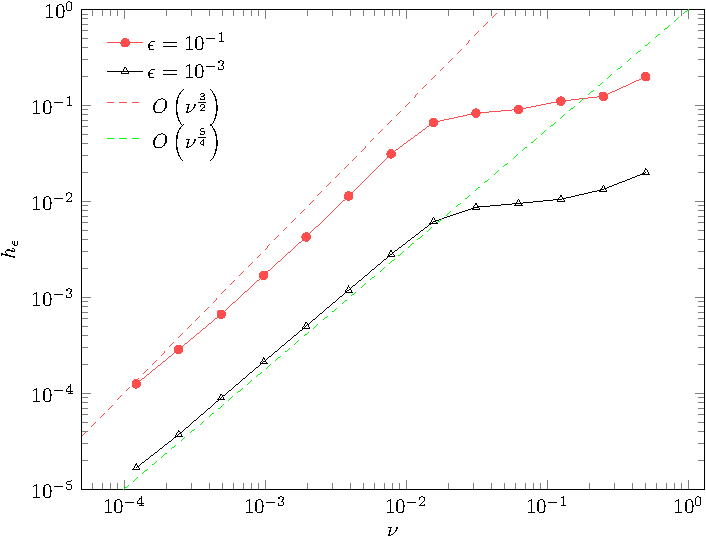
\includegraphics[height=0.35\textwidth]{pics_frequency_domain/h_nu.pdf}
&
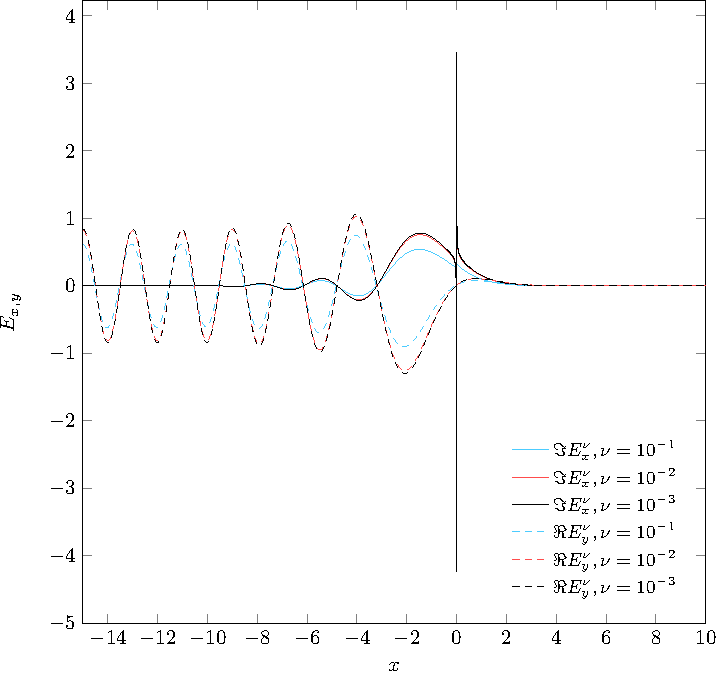
\includegraphics[height=0.35\textwidth]{pics_frequency_domain/res_sol.pdf}
\end{tabular}
\caption{In the left figure the depenence of $h_{\epsilon}$ as defined by (\ref{eq:def_epsilon}) on $\nu$ is demonstrated. 
In the right figure we show the computed solutions for the problem with parameters in Table \ref{tab:parameters} for different values of $\nu$. }
\label{fig:dependence}
\end{figure}
\mrev{We can see that the estimate (\ref{eq:estimate_h}) is pessimistic compared to the one suggested by (\ref{eq:def_epsilon}), 
at least for given values of $\epsilon$ and for a chosen range of $\nu>0$.}


\begin{remark}
It can be shown that $\|E^{\nu}_{x}\|_{L_{2}(\Omega)}\leq \frac{C}{\sqrt{\nu}},\; C>0$, 
and thus the relative error control
\bealn
 \frac{\|E^{\nu}_{x}-E^{\nu,h}_{x}\|_{L_{2}(\Omega)}}{\|E^{\nu}_{x}\|_{L_{2}(\Omega)}}\leq \epsilon
\eealn
 is ensured by choosing $h$ as $\beta_{\epsilon}\nu^{\frac{3}{4}}$.
\end{remark}

\FloatBarrier
\paragraph{Condition Number}
In Figure \ref{fig:small_nu} we demonstrate the dependence of the condition number of the matrix of the system (\ref{eq:simple_system}) 
on $\nu$, for several values of $h$.
\begin{figure}
\begin{tabular}{cc}
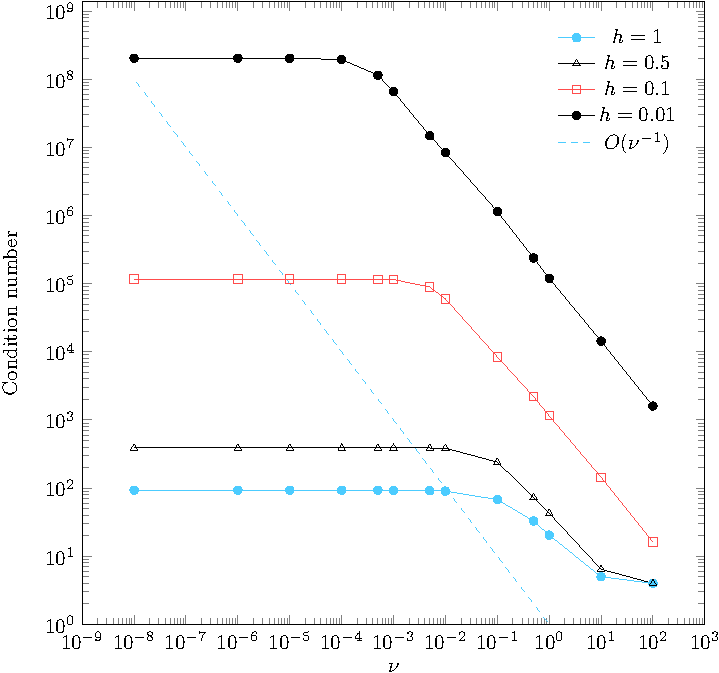
\includegraphics[height=0.35\textwidth]{pics_frequency_domain/fig_cond_num.pdf}&
 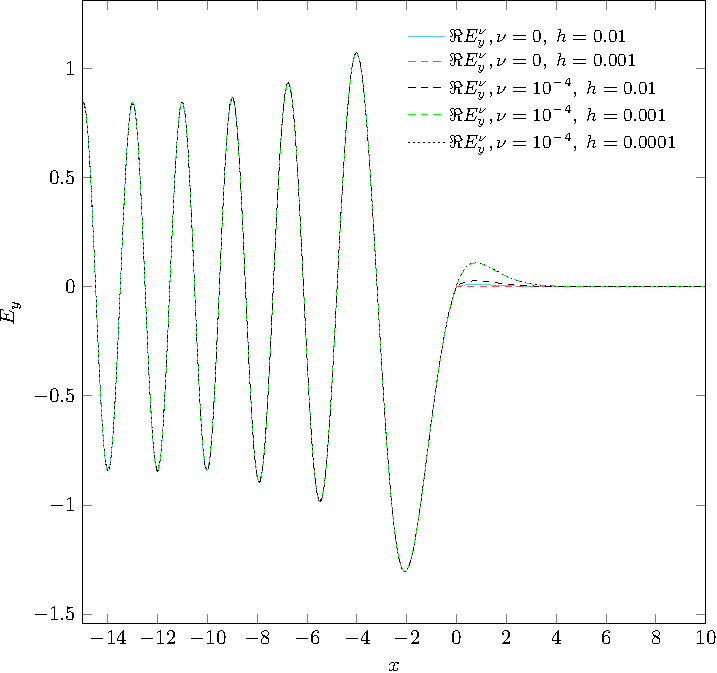
\includegraphics[height=0.35\textwidth]{pics_frequency_domain/ey_resonance.pdf}
 \end{tabular}
 \caption{
 The left plot demonstrates the dependence of the condition number of the system (\ref{eq:simple_system}) on $\nu$, for different values of $h$ (the condition 
 number for $\nu=0$ is not shown, however, for all values of $h$ as shown in the plot, the matrix was non-singular even for $\nu=0$). 
 The right plot shows $E_{y}^{\nu}$ computed on different meshes for small $\nu$. It can be seen that for meshes that are coarse 
 with respect to $\nu$ (e.g. $\nu=10^{-4}, \; h=10^{-2}$, or $\nu=0,\; h=10^{-2}$), the computed solution seems to be only piecewise-continuous in $\nu$, 
 while for finer meshes and $\nu>0$ the solution seems to be smooth. It can be also seen that for $h=10^{-2}$ and $h=10^{-3}$ the solutions 
 computed for $\nu=0$ are almost indistinguishable.}
 \label{fig:small_nu}
\end{figure}
%\begin{table}[ht!]
%\begin{tabular}{c|ccccccccc}
%\diagbox[width=10em]{$h$}{$\nu$}& 100 & 10 & 1 & 0.1 & 1e-2 & 1e-3 & 1e-4 & 1e-8 & 0\\
% \hline
%1 & 3.9634&4.3787 &4.987&36.949&42.394& 42.757 &42.79&42.793&42.793\\
%\hline
%0.5&      3.9931& 6.87&48.473 & 168.41  &207.34  & 209.63 & 209.83 & 209.85&  209.85\\
%\hline
% 0.1&      16.09  &     159.56  &     1146.1   &    8304.1   &     19169  &      20270   &     20344   &     20352   &     20352\\
% \hline
%0.05&      64.046  &     637.18  &     4686.2   &     38876 &  1.4e5 &  1.58e5 &   1.58e5 &  1.58e5 &  1.58e5\\
%\hline
% 0.01&       1600    &   15921 & 1.2e5  & 1.1e6 & 8.3e6  & 1.8e7   & 1.93e7  & 1.93e7  & 1.93e7\\
%\end{tabular}
%\caption{The condition number of the matrix of the system (\ref{eq:simple_system}) for different values of $\nu$ and $h$. }
%\label{tab:cond_number}
%\end{table}
Remarkably, for $\nu=0$ the computed matrices are not singular. We do not know the exact reason for this.
As an additional illustration, we compare the solutions for very small $\nu$ and $\nu=0$ for different meshes in Fig.~\ref{fig:small_nu}. 

\FloatBarrier

\subsection{A validation of the semi-lagrangian scheme}

We show the results of very basic simulations that the numerical strategy 
based on co-localised semi-lagrangian discretization is valid even for the resonant 
case.
The numerical tests have been kept to a minimum since much more are needed to fully validate
the concept.

The setting of the numerical results of figure \ref{fig:vasl}
is the following. We use a 7th order semi-lagrangian scheme, and the CFL is $\nu=0.5$.
The Pike is the hybrid resonance, visible on $E_x$ and $u_x$.
The total energy $\mathcal E(t)$ is the physical energy. 
The comparison with figures \ref{fig:dependence} and \ref{fig:resonance_nus_ey_x} show that the 
singular nature of the resonant is captured by this new scheme without any doubt.

\begin{figure}{h}
	\begin{center}
		\begin{tabular}{ccc}
			\includegraphics[angle=-90,width=5.cm]{pics_semilagrange/Ey_moit.eps}
			&
			\includegraphics[angle=-90,width=5.cm]{pics_semilagrange/Hz_moit.eps} &
			\includegraphics[angle=-90,width=5.cm]{pics_semilagrange/Ex_moit.eps}
			\\
			$E_y$ & $H_z$  & $E_x^\nu$ \\
			%\hline
			\hline
			\includegraphics[angle=-90,width=5.cm]{pics_semilagrange/uy_moit.eps}
			&
			\includegraphics[angle=-90,width=5.cm]{pics_semilagrange/normes_moit.eps}
			&
			\includegraphics[angle=-90,width=5.cm]{pics_semilagrange/ux_moit.eps}
			\\      
			$u_y$ & $t\mapsto \mathcal E(t)$ & $u_x^\nu$  \\
			
			%\includegraphics[width=4.cm]{cap14.png} 
			\\
			
			
		\end{tabular}   \end{center}
		\caption{An antenna sends a time harmonic wave on the left. The medium is propagative
			on the left and non propagative
			on the right. The resonance is visible on $E_x$ and $u_x$. The time of the simulation is $T=2000$. The number of cells
			is typically 10000 to reach convergence.}
		\label{fig:vasl}
	\end{figure}


%\subsubsection{No-Resonance Case}
%We choose the parameters so that in the frequency domain, for the limiting amplitude problem, $\hat{E}_{2}$ satisfies 
%the Airy equation \cite{}. 

%We set $\omega_c=0$ (thus $\delta(x)=0$), $\omega=1$ (hence $\alpha(x)=1-N_e(x)$), 
%choose the domain as $[-0.5, 10]$ and set the electron density $N_e(x)=1+x$. Importantly, $N_e(x)>0$ on the whole interval.
%The boundary conditions in (\ref{eq:bcs}) are chosen as $G=Ai'(0.5)$. 
%In all the experiments in this section the CFL number was chosen to be equal to 0.5.


%First let us fix $\nu=1e-2$. 
%To demonstrate that the limiting amplitude principle indeed holds, we fix a point $x=x_c$ 
%inside the domain $(-L,\; H)$ and plot the dependence of the solution $E_{y}^{\nu}(x_c,t), \; \hat{E}_2^{\nu}(x_c)\mathrm{e}^{it}$ 
%on time $t$ for a range of $t\gg 1$ in Figure \ref{fig:nu1e2_harmon}.  

\subsection{Limiting Amplitude and Limiting Absorption Principle}
In this section we perform several numerical experiments,
with the normalization chosen as $\epsilon_0=\mu_0=1$, $\omega=c=1$. 
Also, we set $m_e=1$ and $e=-1$. From this it follows that $w_c=-B_0$ and $w_p^2=N_e$. 
We consider the following two cases:
\begin{itemize}
 \item case $N_e\neq \operatorname{const}$, no resonance
 \item case $N_e\neq \operatorname{const}$, resonance
\end{itemize}
For every fixed absorption rate $\nu$, in the time domain we choose the boundary conditions of the form
\begin{align}
\label{eq:bcs}
\left.\partial_t H\right|_{x=-L}&=-\left.\partial_x E_y\right|_{x=-L}=G\sin(t),\; G\in \mathbb{R}, \\
 \nonumber
 \left.\partial_t H\right|_{x=H}&=0,
\end{align}
and zero initial conditions, and in the frequency domain
\begin{align*}
 \left.\partial_x \hat{E}_y\right|_{x=-L}&=G,\\
 \left.\partial_x \hat{E}_y\right|_{x=H}&=0.
\end{align*}
We compute the solution $\mathbf{E}^{\nu}(t)$ for large $t$ in the time domain (the solution computed numerically at the time step $n$ is denoted by $\mathbf{E}^{\nu}_{n}$), and the solution $\hat{\mathbf{E}}^{\nu}$ in the frequency domain. 
Our goal is to check whether
\begin{align*}
\lim_{t\rightarrow+\infty}\mathbf{E}^{\nu}(t)=\Im\left(\hat{\mathbf{E}}^{\nu}\exp(it)\right).
\end{align*}

\subsubsection{No-Resonance Case}
We choose the parameters so that in the frequency domain, for the limiting amplitude problem, $\hat{E}_{2}$ satisfies 
the Airy equation (\ref{}). 

We set $\omega_c=0$ (thus $\delta(x)=0$), $\omega=1$ (hence $\alpha(x)=1-N_e(x)$), 
choose the domain as $[-0.5, 10]$ and set the electron density $N_e(x)=1+x$. Importantly, $N_e(x)>0$ on the whole interval.
The boundary conditions in (\ref{eq:bcs}) are chosen as $G=Ai'(0.5)$. 
In all the experiments in this section the CFL number was chosen to be equal to 0.5.


First let us fix $\nu=1e-2$. 
To demonstrate that the limiting amplitude principle indeed holds, we fix a point $x=x_c$ 
inside the domain $(-L,\; H)$ and plot the dependence of the solution $E_{2}^{\nu}(x_c,t), \; \hat{E}_2^{\nu}(x_c)\mathrm{e}^{it}$ 
on time $t$ for a range of $t\gg 1$ in Figure \ref{fig:nu1e2_harmon}.  

\begin{figure}[htb]
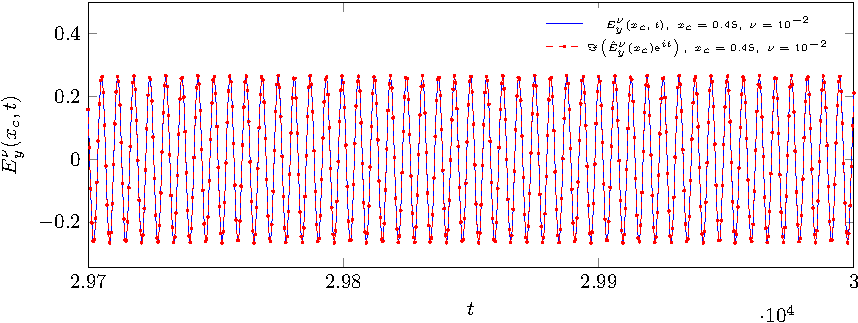
\includegraphics[width=0.9\textwidth]{figure_nu1e2-crop.pdf}
 \label{fig:nu1e2_harmon}
\end{figure}

In Figure \ref{fig:nu1e2_harmon2} (left figure) we compare this solution to the computed $\hat{E}_2^{\nu}\mathrm{e}^{it}$, for
fixed values of $t$. Both solutions appear to be in close agreement. 
\begin{figure}[htb]
 \begin{tabular}{ll}
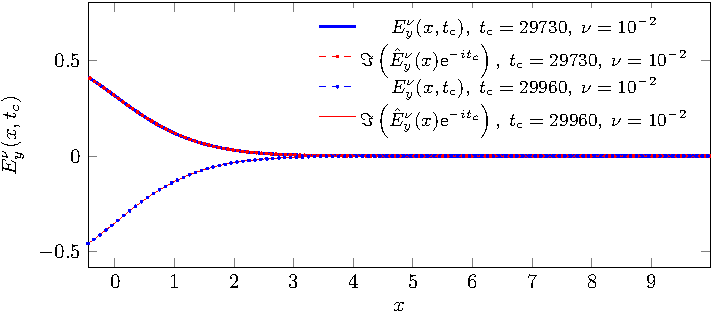
\includegraphics[width=0.5\textwidth]{figure_nu1e2_2-crop.pdf}
&
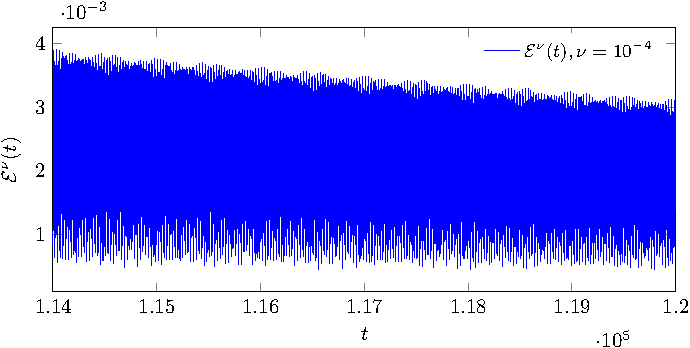
\includegraphics[width=0.5\textwidth]{figure_error_nu1e4-crop.pdf}\\
\end{tabular}
\caption{In the left figure we show the solution to (\ref{}) for $\nu=10^{-2}$, for two fixed moment of times. In the right figure 
the dependence of the error (\ref{eq:error}) on time for $\nu=10^{-4}$ is demonstrated. 
We can see that the error is decreasing.}
 \label{fig:nu1e2_harmon2}
\end{figure}
The computed $L_2$ error
\begin{align}
\label{eq:error}
\mathcal{E}(t)=\|\Im\left(\hat{E}_y^{\nu}\exp(it)\right)-E_y^{\nu}(t)\|_{L_{2}(-L;H)}.
\end{align}
for $\nu=1e-2$ did not exceed $1.1e-3$ for values of $t\in \left(28501,  30000\right)$. 

Figure show the solutions at fixed time steps for $\nu=1e-4$. As before, 
to demonstrate that the limiting amplitude principle indeed holds, we fix a point $x=x_c$ 
inside the domain $(-L,\; H)$ and plot 
the dependence of the solution $E_{2}^{\nu}(x_c,t)$ on time $t$ for a range of $t\gg 1$. 
The error (\ref{eq:error}) for $\nu=1e-4$ at the time interval $[228000.05,\; 240000.05]$ does not exceed 2.8e-4. 
One of our observations was that for smaller $\nu$ one requires more time steps to achieve the limiting amplitude solution, 
c.f. e.g. Figure \ref{fig:nu1e2_harmon2}. 
We were not able to obtain the limiting amplitude solution for $t<3\cdot 10^{4}$, unlike in the case of $\nu=10^{-2}$. 
For example, for $\nu=1e-6$ we were not able to reach the limiting amplitude solution even on the time interval $t\leq 1.92e6$, 
see Figure \ref{fig:nu1e4_harmon}. 
\begin{figure}
\begin{tabular}{c}
 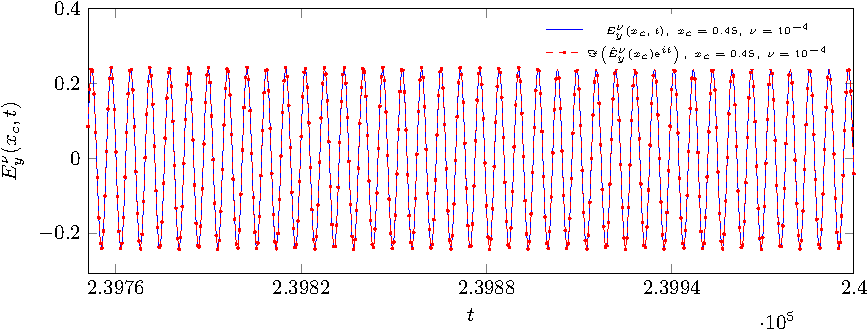
\includegraphics[width=\textwidth]{figure_nu1e4-crop.pdf}\\
 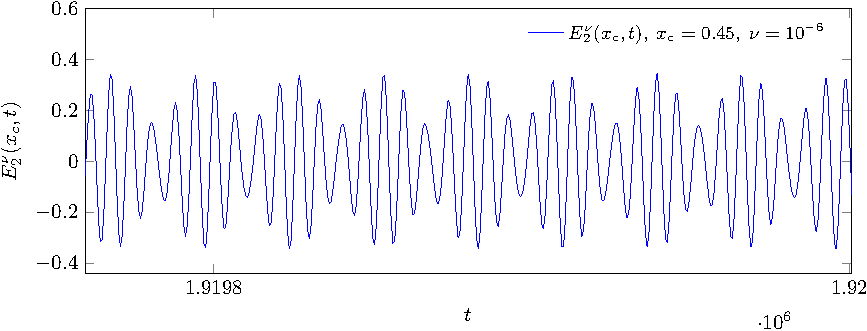
\includegraphics[width=\textwidth]{figure_nu1e6-crop.pdf}\\
\end{tabular}
\caption{In the upper figure we plot the dependence of the solution $E_{2}^{\nu}(x_c,t)$ on time $t$, with $\nu=10^{-4}$ and $x_c=0.45$. 
In the lower figure we show the solution for $\nu=10^{-6}$ at the same point $x_c$, for larger times. As we can see, for 
$\nu=10^{-4}$ the limiting amplitude solution was reached for large $t$. For $\nu=10^{-6}$ we were not able 
to obtain the limiting amplitude solution even for $t\approx 1.9e6$. }
  \label{fig:nu1e4_harmon}
\end{figure}

\subsubsection{Resonance Case}
\label{sec:resn}
For the resonance case, we choose the parameters as given in Table \ref{tab:parameters_resonance}.
\begin{table}[htb!]
\begin{tabular}{c|c}
Parameter & Value \\
\hline
$L$ & 5\\
$H$ & 19\\
$\omega_c$ &  $\sqrt{0.5}$\\
$N_e(x)$ &  $\left\{
 \begin{array}{cc}
  0.25, & x<-0.5,\\
  \frac{1+x}{2}, & x\geq -0.5, x\leq 9\\
  5, & x>9.
 \end{array}\right.$\\
 $G$ as in (\ref{eq:bcs}) & 0.11 \\
\end{tabular}
\label{tab:parameters_resonance}
\caption{Parameters for numerical simulations in Section \ref{sec:resn}}
\end{table}
Since $\alpha(x)=(1-2N_e(x))$, $\alpha(0)=0$. Clearly, $\delta(0)\neq 0$ (resonance case).

The results for $\nu=10^{-2}$ (chosen as a parameter both in frequency and time domain) 
are shown in Figure \ref{fig:resonance_nu1e2} and for $\nu=10^{-3}$ in Figure \ref{resonance_nu1e3}. 
\begin{figure}
 
 \caption{In the }
 \label{fig:resonance_nu1e2}
\end{figure}


For $\nu=10^{-6}$, like in the previous case, we were not able to obtain the limiting amplitude solution in the time domain.




\section{Conclusions}
In this work we considered the frequency- and the time-domain formulations of the $X$-mode Maxwell equations. 
In particular, we proved the well-posedness of the respective regularized (with the help of 
the absorption parameter $\nu$) variational formulation, as 
well as studied the convergence of the finite element method for the problem with the resonance. 
The piecewise-constant FEM approximates the resonant solution rather well, at least for moderate values of $\nu$, 
however, the discretization size should be chosen roughly proportional to $\nu^{\frac{3}{2}}$, in order to obtain an accurate discretization.
Indeed, it would be interesting to look at the convergence of the adaptive finite elements for this kind of problems. 
Another unanswered question is the well-posedness of the discrete problem when the continuous problem is ill-posed. We have 
demonstrated that while the condition number of the FEM matrix grows, the matrix remains always invertible, even for $\nu=0$. 

We proposed two different schemes for solving the time-dependent problem. Our numerical experiments demonstrate that both of them capture the singular behaviour of the solutions in the resonant case.

The other part of the experiments concerned the equivalence of the limiting absorption and limiting amplitude solutions. We have shown 
that for small $\nu$ and large times the solution computed in the time domain is close to the solution predicted by the limiting amplitude principle; as 
$\nu\rightarrow 0$, the solution oscillates harmonically as $t\rightarrow +\infty$, however, we were not able to compute the limiting amplitude solution for very 
small values of $\nu$. 


\begin{thebibliography}{99}
	\bibitem{abramowitz_stegun} Abramowitz M. and Stegun I. A., eds. (1972). Handbook of Mathematical Functions with Formulas, Graphs, and Mathematical Tables. New York: Dover Publications.
	Handbook of mathematical functions
	\bibitem{brenner} Brenner, S. C. and Scott, R. (2008). The mathematical theory of finite element methods (Vol. 15). Springer.
\bibitem{cedar}
Charles, F., Despr\'es, B., Merhenberg, M, 
Enhanced convergence estimates for semi-lagrangian schemes Application to the Vlasov-Poisson equation, SIAM J. Numer. Anal. 2013, 51(2), 840-863.

\bibitem{stable_yee_plasma_current} Da Silva, F., Campos-Pinto, M., Després, B., and Heuraux, S. (2014). Stable coupling of the Yee scheme with a linear current model.

\bibitem{compfluids}
S. Del Pino, B. Despr\'es, P. Hav\'e, H. Jourdren, and P. F. Piserchia. 3D finite
volume simulation of acoustic waves in the earth atmosphere.
Comput. \&
Fluids, 38(4):765-777, 2009.

\bibitem{reflectometers_2006} Da Silva, F., Heuraux, S and  Manso, M. (2006). Developments on reflectometry simulations for fusion plasmas: application to ITER position reflectometers. Journal of plasma physics, 72(06), 1205-1208.

\bibitem{reflectometers_2010}Da Silva, F., Heuraux, S., Gusakov, E. Z., and Popov, A. (2010). A Numerical Study of Forward-and Backscattering Signatures on Doppler-Reflectometry Signals. Plasma Science, IEEE Transactions on, 38(9), 2144-2149.

\bibitem{Despres_2014} Després, B., Imbert-Gérard, L. M. and Weder, R. (2014). Hybrid resonance of Maxwell's equations in slab geometry. Journal de Mathématiques Pures et Appliquées, 101(5), 623-659.

\bibitem{Dumont_2005} Dumont, R. J., Phillips, C. K., and Smithe, D. N. (2005). Effects of non-Maxwellian species on ion cyclotron waves propagation and absorption in magnetically confined plasmas. Physics of Plasmas (1994-present), 12(4), 042508.

\bibitem{Freidberg_2007} Freidberg, J. P. (2007). Plasma physics and fusion energy. Cambridge university press.


\bibitem{phdhattori}
T. Hattori, T. (2014).
D\'ecomposition de domaine pour la simulation Full-Wave dans un plasma froid.
Ph.D. Thesis, Universit\'e de
Lorraine.

\bibitem{LMIG_thesis} Imbert-Gérard, L. M. (2013). Analyse mathématique et numérique de problèmes d'ondes apparaissant dans les plasmas magnétiques (Doctoral dissertation, Université Pierre et Marie Curie-Paris VI).




\bibitem{simon}
Simon Labrunie, Pierre Bertrand, Jean-Rodolphe Roche, Aurore Back,
Takashi Hattori, 
Electromagnetic wave propagation and absorption in
magnetised plasmas: variational formulations and
domain decomposition, Hal preprint 2014, https://hal.archives-ouvertes.fr/hal-01075137.




\bibitem{Morawetz} Morawetz, C. S. (1962). The limiting amplitude principle. Communications on Pure and Applied Mathematics, 15(3), 349-361.

\bibitem{Stix} Stix, T. H. (1992). Waves in plasmas. Springer.
\bibitem{Xu_2006}Xu, L., ans Yuan, N. (2006). FDTD formulations for scattering from 3-D anisotropic magnetized plasma objects. Antennas and Wireless Propagation Letters, IEEE, 5(1), 335-338.
\end{thebibliography}

\end{document}
